%% Copernicus Publications Manuscript Preparation Template for LaTeX Submissions
%% ---------------------------------
%% This template should be used for copernicus.cls
%% The class file and some style files are bundled in the Copernicus Latex Package, which can be downloaded from the different journal webpages.
%% For further assistance please contact Copernicus Publications at: production@copernicus.org
%% https://publications.copernicus.org/for_authors/manuscript_preparation.html

%% copernicus_rticles_template (flag for rticles template detection - do not remove!)

%% Please use the following documentclass and journal abbreviations for discussion papers and final revised papers.

%% 2-column papers and discussion papers
\documentclass[, manuscript]{copernicus}



%% Journal abbreviations (please use the same for preprints and final revised papers)

% Advances in Geosciences (adgeo)
% Advances in Radio Science (ars)
% Advances in Science and Research (asr)
% Advances in Statistical Climatology, Meteorology and Oceanography (ascmo)
% Annales Geophysicae (angeo)
% Archives Animal Breeding (aab)
% Atmospheric Chemistry and Physics (acp)
% Atmospheric Measurement Techniques (amt)
% Biogeosciences (bg)
% Climate of the Past (cp)
% DEUQUA Special Publications (deuquasp)
% Drinking Water Engineering and Science (dwes)
% Earth Surface Dynamics (esurf)
% Earth System Dynamics (esd)
% Earth System Science Data (essd)
% E&G Quaternary Science Journal (egqsj)
% EGUsphere (egusphere) | This is only for EGUsphere preprints submitted without relation to an EGU journal.
% European Journal of Mineralogy (ejm)
% Fossil Record (fr)
% Geochronology (gchron)
% Geographica Helvetica (gh)
% Geoscience Communication (gc)
% Geoscientific Instrumentation, Methods and Data Systems (gi)
% Geoscientific Model Development (gmd)
% History of Geo- and Space Sciences (hgss)
% Hydrology and Earth System Sciences (hess)
% Journal of Bone and Joint Infection (jbji)
% Journal of Micropalaeontology (jm)
% Journal of Sensors and Sensor Systems (jsss)
% Magnetic Resonance (mr)
% Mechanical Sciences (ms)
% Natural Hazards and Earth System Sciences (nhess)
% Nonlinear Processes in Geophysics (npg)
% Ocean Science (os)
% Polarforschung - Journal of the German Society for Polar Research (polf)
% Primate Biology (pb)
% Proceedings of the International Association of Hydrological Sciences (piahs)
% Safety of Nuclear Waste Disposal (sand)
% Scientific Drilling (sd)
% SOIL (soil)
% Solid Earth (se)
% The Cryosphere (tc)
% Weather and Climate Dynamics (wcd)
% Web Ecology (we)
% Wind Energy Science (wes)

% Pandoc citation processing

% The "Technical instructions for LaTex" by Copernicus require _not_ to insert any additional packages.
% 
% tightlist command for lists without linebreak
\providecommand{\tightlist}{%
  \setlength{\itemsep}{0pt}\setlength{\parskip}{0pt}}


%%\usepackage{booktabs}
\usepackage{longtable}
\usepackage{array}
\usepackage{multirow}
\usepackage{wrapfig}
\usepackage{float}
\usepackage{colortbl}
\usepackage{pdflscape}
\usepackage{tabu}
\usepackage{threeparttable}
\usepackage{threeparttablex}
\usepackage[normalem]{ulem}
\usepackage{makecell}
\usepackage{xcolor}
%
\begin{document}


\title{A detailed streamflow and groundwater salinity dataset for
Muttama Creek Catchment, NSW, Australia}


\Author[1]{R. Willem}{Vervoort}
\Author[1]{Floris}{van Ogtrop}
\Author[1]{Mina}{Tambrchi}
\Author[1]{Farzina}{Akter}
\Author[1]{Alexander}{Buzacott}
\Author[1]{Jason}{Lessels}
\Author[1]{James}{Moloney}
\Author[1]{Niranjan}{Wimalathunge}
\Author[1]{Dipangkar}{Kundu}
\Author[1]{Feike}{Dijkstra}
\Author[1]{Thomas}{Bishop}


\affil[1]{Sydney Institute of Agriculture, The University of Sydney, NSW
2006}

\runningtitle{Muttama Creek Salinity Data Set}

\runningauthor{Vervoort et al.}


\correspondence{R. Willem\ Vervoort\ (willem.vervoort@sydney.edu.au)}



\received{}
\pubdiscuss{} %% only important for two-stage journals
\revised{}
\accepted{}
\published{}

%% These dates will be inserted by Copernicus Publications during the typesetting process.


\firstpage{1}

\maketitle


\begin{abstract}
Dryland salinity remains a major natural resource management concern,
specifcially in Australia, but also globally. However, a lack of
detailed space-time data sets with observations of stream and
groundwater salinity has limited further understanding of the range of
processes that can lead to dryland salinity problems in landscapes. The
aim of this study is to report on the open data available as a result of
a 10-year data collection effort in a subcatchment of the Murrumbidgee
catchment in New South Wales, Australia. Over a 10 year period a series
of different sampling campaigns has resulted in a large dataset with
hydrogeochemical data which includes both in-situ (field) data and post
laboratory analysis of major anions and cations. The data set covers 23
groundwater sample sites and 37 surface water sites. Because the data
was collected by four distinct groups and over many years we analyse if
this has caused a bias in the dataset. In addition we show the major
spatial and temporal trends to provide an overview of the dataset and
analyse any posible biases. The dataset is made open access to encourage
further research and the basic description already shows the richness of
the collected data and opportunities for further research.
\end{abstract}


\copyrightstatement{The author's copyright for this publication is
transferred to institution/company.}


\introduction

Dryland and irrigation salinity has long been a major natural resource
management concern in Australia
\citep{Jolly2001, White2009, Scanlon2007, Walker2002, Finlayson2010}.
The success of management of salinity, while extensively documented, has
remained patchy \citep{Leblanc2012}. As a result, the volume of research
and number of publications in this area has decreased significantly in
recent years (Figure \ref{fig:SalinityPapers}). This is partly due to
the effect of the millenium drought on groundwater levels and
consequently salinity \citep{Mcfarlane2016}, but this is also because of
the increased understanding that salinity processes can vary
substantially across the landscape \citep{Conyers2008} and that the
processes of salt delivery to the stream also varies in the landscape
\citep{Summerell2006, Hughes2007} and is dependent on landscape
characteristics \citep{vanDijk2008, Dalhaus2010}.

\begin{figure}
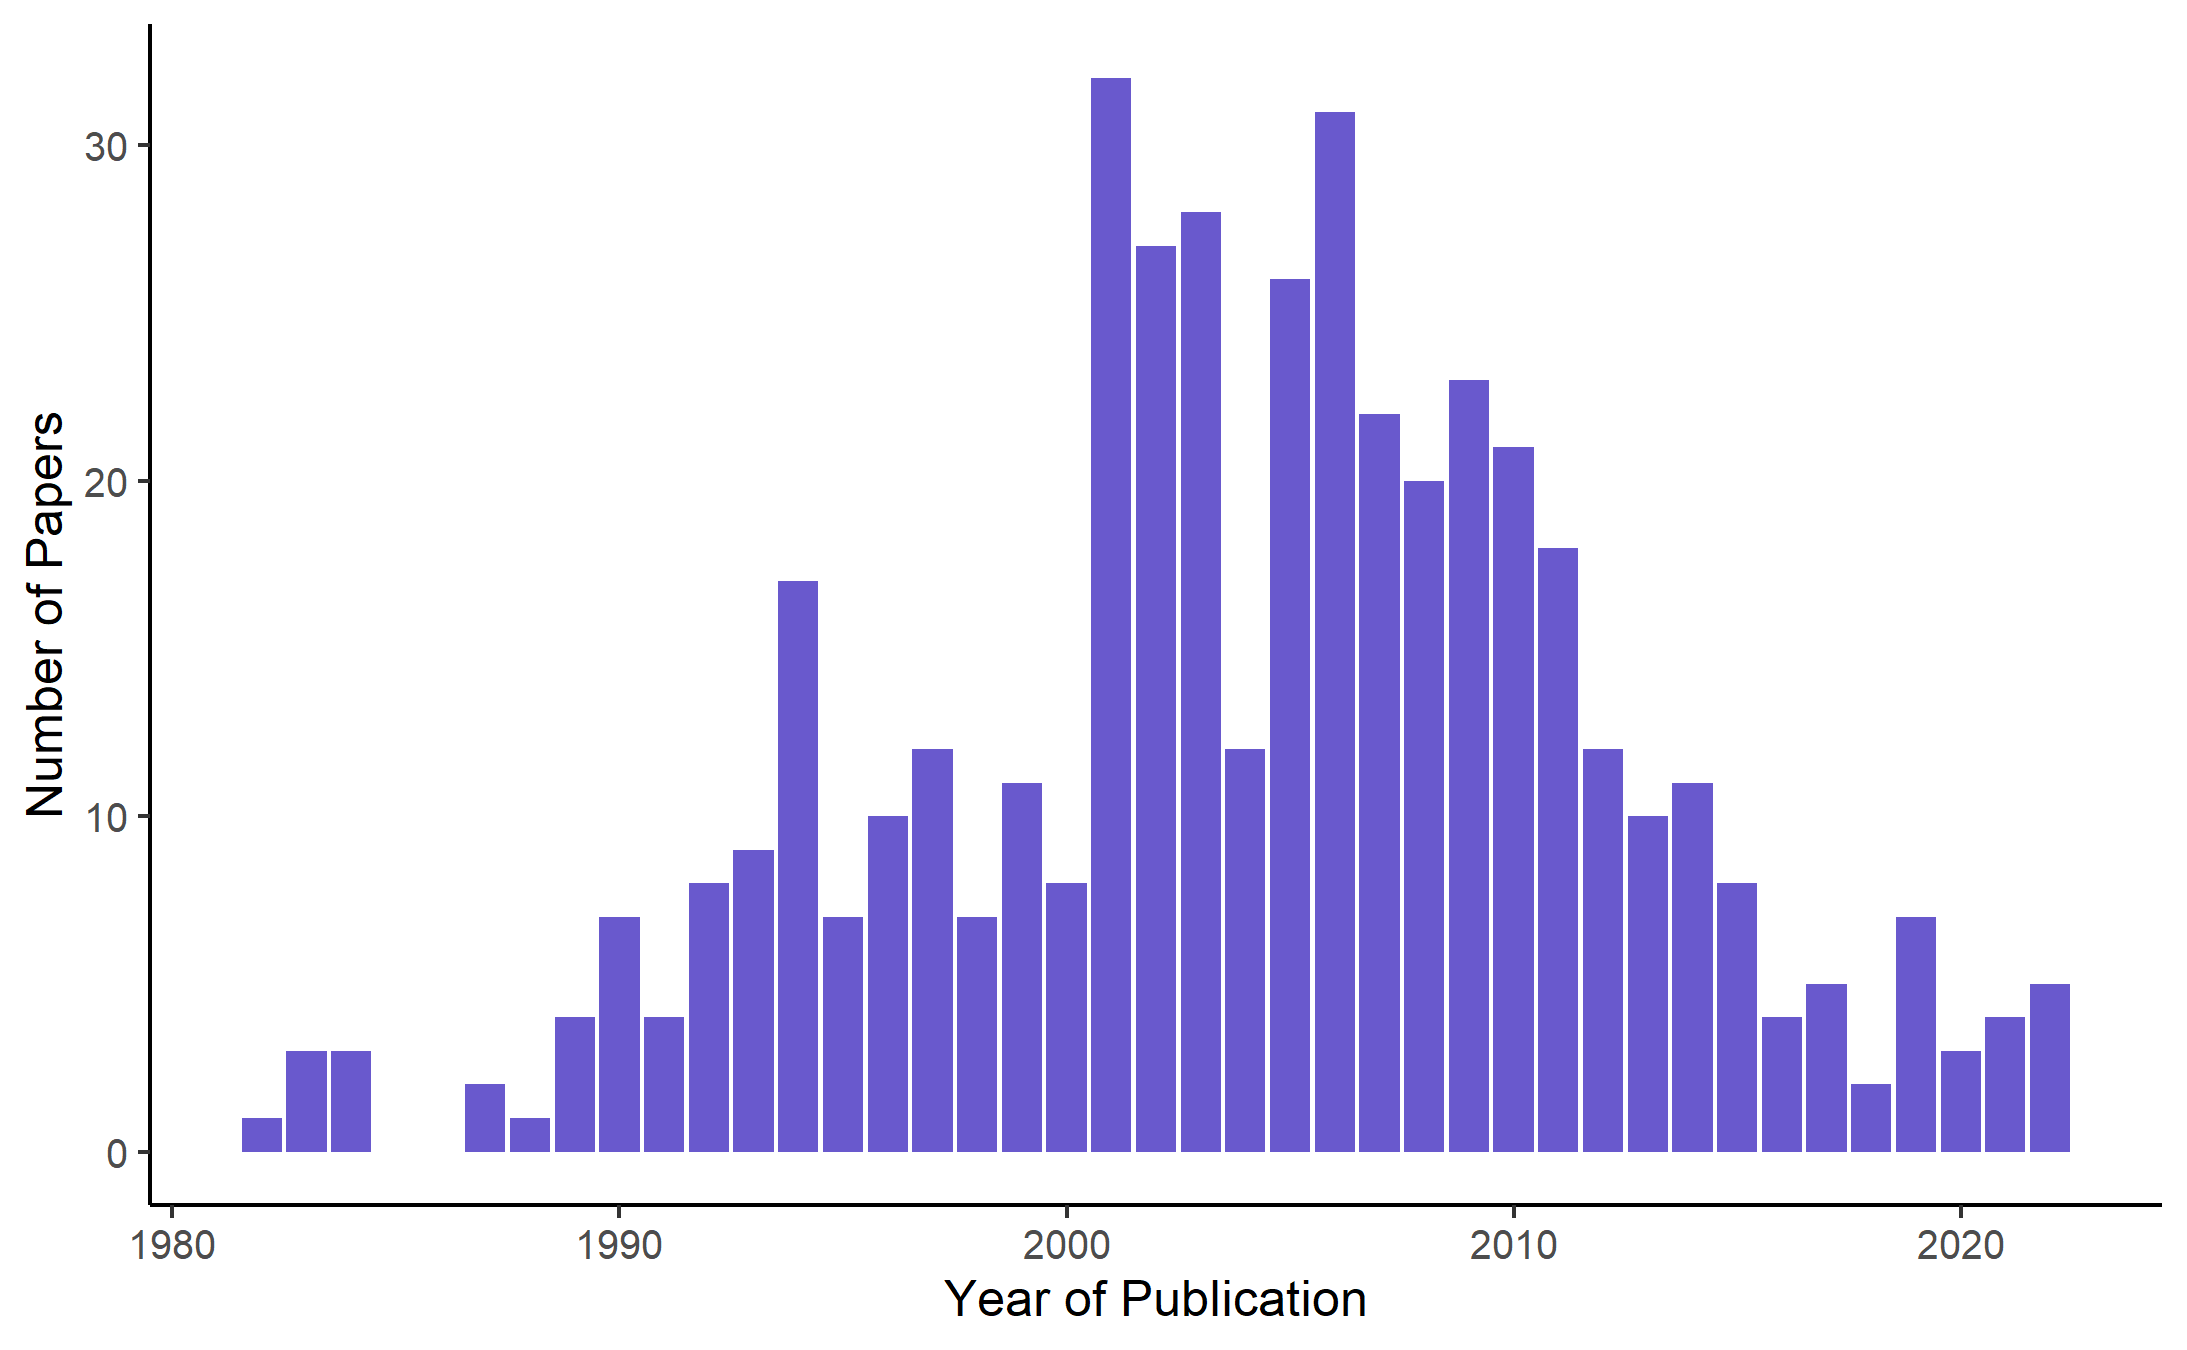
\includegraphics[width=0.9\linewidth]{Figures/Dryland Salinity Papers} \caption{Number of papers on the Web of Science related to the search terms (Dryland Salinity) AND Australia 1980 - 2022}\label{fig:SalinityPapers}
\end{figure}

The poor spatial and timescale distribution of water quality datasets
has long been an obstacle to measuring trends in salinity. Studies such
as Jolly et. al. \citeyearpar{Jolly2001} and White et. al
\citeyearpar{White2009} used large historical datasets to detect
broadscale trends over large periods throughout the Murray Darling Basin
(MDB). This work identified that southern and eastern dryland region in
the Murray Darling Basin have rising salinity trends that were worse in
areas of low rainfall \citep{White2009, Jolly2001}. However, the ion
composition varied greatly throughout the MDB \citep{White2009}. More
specifically, Conyers et al. \citeyearpar{Conyers2008} tried to isolate
which areas of land in the Murrumbidgee catchment acted as sources of
salinity, as well as whether this was predominantly marine cyclic salts
(NaCl) as previously assumed, or whether salts from mineral weathering
were also involved (e.g.~Ca, Mg, HCO\textsubscript{3}). While both can
be measured using conventional methods such as EC, a rise in marine
cyclic salts can be a major source of osmotic stress, whereas mineral
weathering salts are far less harmful and more likely to precipitate at
reasonably low concentrations \citep{Conyers2008}. The ratio of
Cl:HCO\textsubscript{3} ions was identified as the best indicator of the
source of salinity, with Cl\textsuperscript{-} acting as a measure of
marine cyclic salts and HCO\textsubscript{3}\textsuperscript{-} acting
as a measure of mineral weathering salts. The Muttama catchment was
specifically identified as a candidate for future research as ion
concentrations appeared to change from east to west, correlating with
the underlaying mineral types.

It is clear from these examples that detailed spatial and temporal
datasets are key to understanding different hydrogeochemical processes
in the landscape \citep[e.g.][]{Cartwright2010, Dalhaus2010}, but
overall publicly available datasets on dryland salinity in Australia
remain limited to detailed data from small experimental catchments
(\textless{} 100 ha) \citep{Summerell2006, Hughes2007} or sparse
government datasets from official monitoring
(i.e.~\url{https://realtimedata.waternsw.com.au} which tend to be
limited in hydrogeochemical data. Part of this is related to the
sensitivity of the data given the relationship with possible land
values. However, as the understanding of salinity occurrence grows this
argument is less valid. In fact, making data more widely available would
increase the opportunities for research and increase our understanding
of dryland salinity processes.

Without regular and expensive automated sampling, field campaigns to
collect water quality data tend to be ``snapshot'' activities
\citep{Grayson1997, Breuer2015, Lyon2008, Cartwright2010, Lintern2018}
which can be biased due to the over representation of low flow
conditions \citep{Lessels2020}. Even the analyses of substantial
government data bases \citep{Lintern2018} are likely to be biased in
this way. This means that overall there are limited streamflow and
groundwater salinity data sets that combine multiple locations across a
significant time period and that combine a range of flow
characteristics.

The aim of this paper is to present and describe the space time
dimensions and relationships of a complex groundwater and surface water
hydrogeochemistry dataset that was collected over a 10 year period in a
1000km\textsuperscript{2} agricultural catchment in New South Wales,
Australia. The Muttama catchment, which is the focus of this paper,
provides a micro-cosm of groundwater and surface water salinity
variability in Australia. Focusing on a smaller catchment in greater
detail creates opportunities to test whether sources of salinity can be
traced back to specific areas of land.

This paper gives a description of the dataset to facilitate open access
of the dataset, but does not analyse the physicochemical relationships
in the data in detail. This will be analysed in follow-up papers. The
main aim of this paper is to make the data set accessible to other
researchers to encourage further research in this catchment and in
salinity in general.

\section{Methods}

\subsection{Muttama catchment}

Muttama creek sub-catchment (Figure \ref{fig:samplemap}) is located in
the Mid-Murrumbidgee catchment area of NSW in south eastern Australia.
The landscape is undulating with only limited elevation variations (227
- 719 m). Muttama creek flows north-south through the length of the
catchment towards the Murrumbidgee River near Gundagai. The main
township, Cootamundra is located in the upper half of the catchment. The
dominant land use type of this catchment is about 93\% agriculture,
dominated by winter-spring cropping and pasture . Mean annual rainfall
(1891-2017) in the catchment is 653 mm for the Bureau of Meteorology
Landgrove station (station 073022).

\clearpage
\begin{figure}
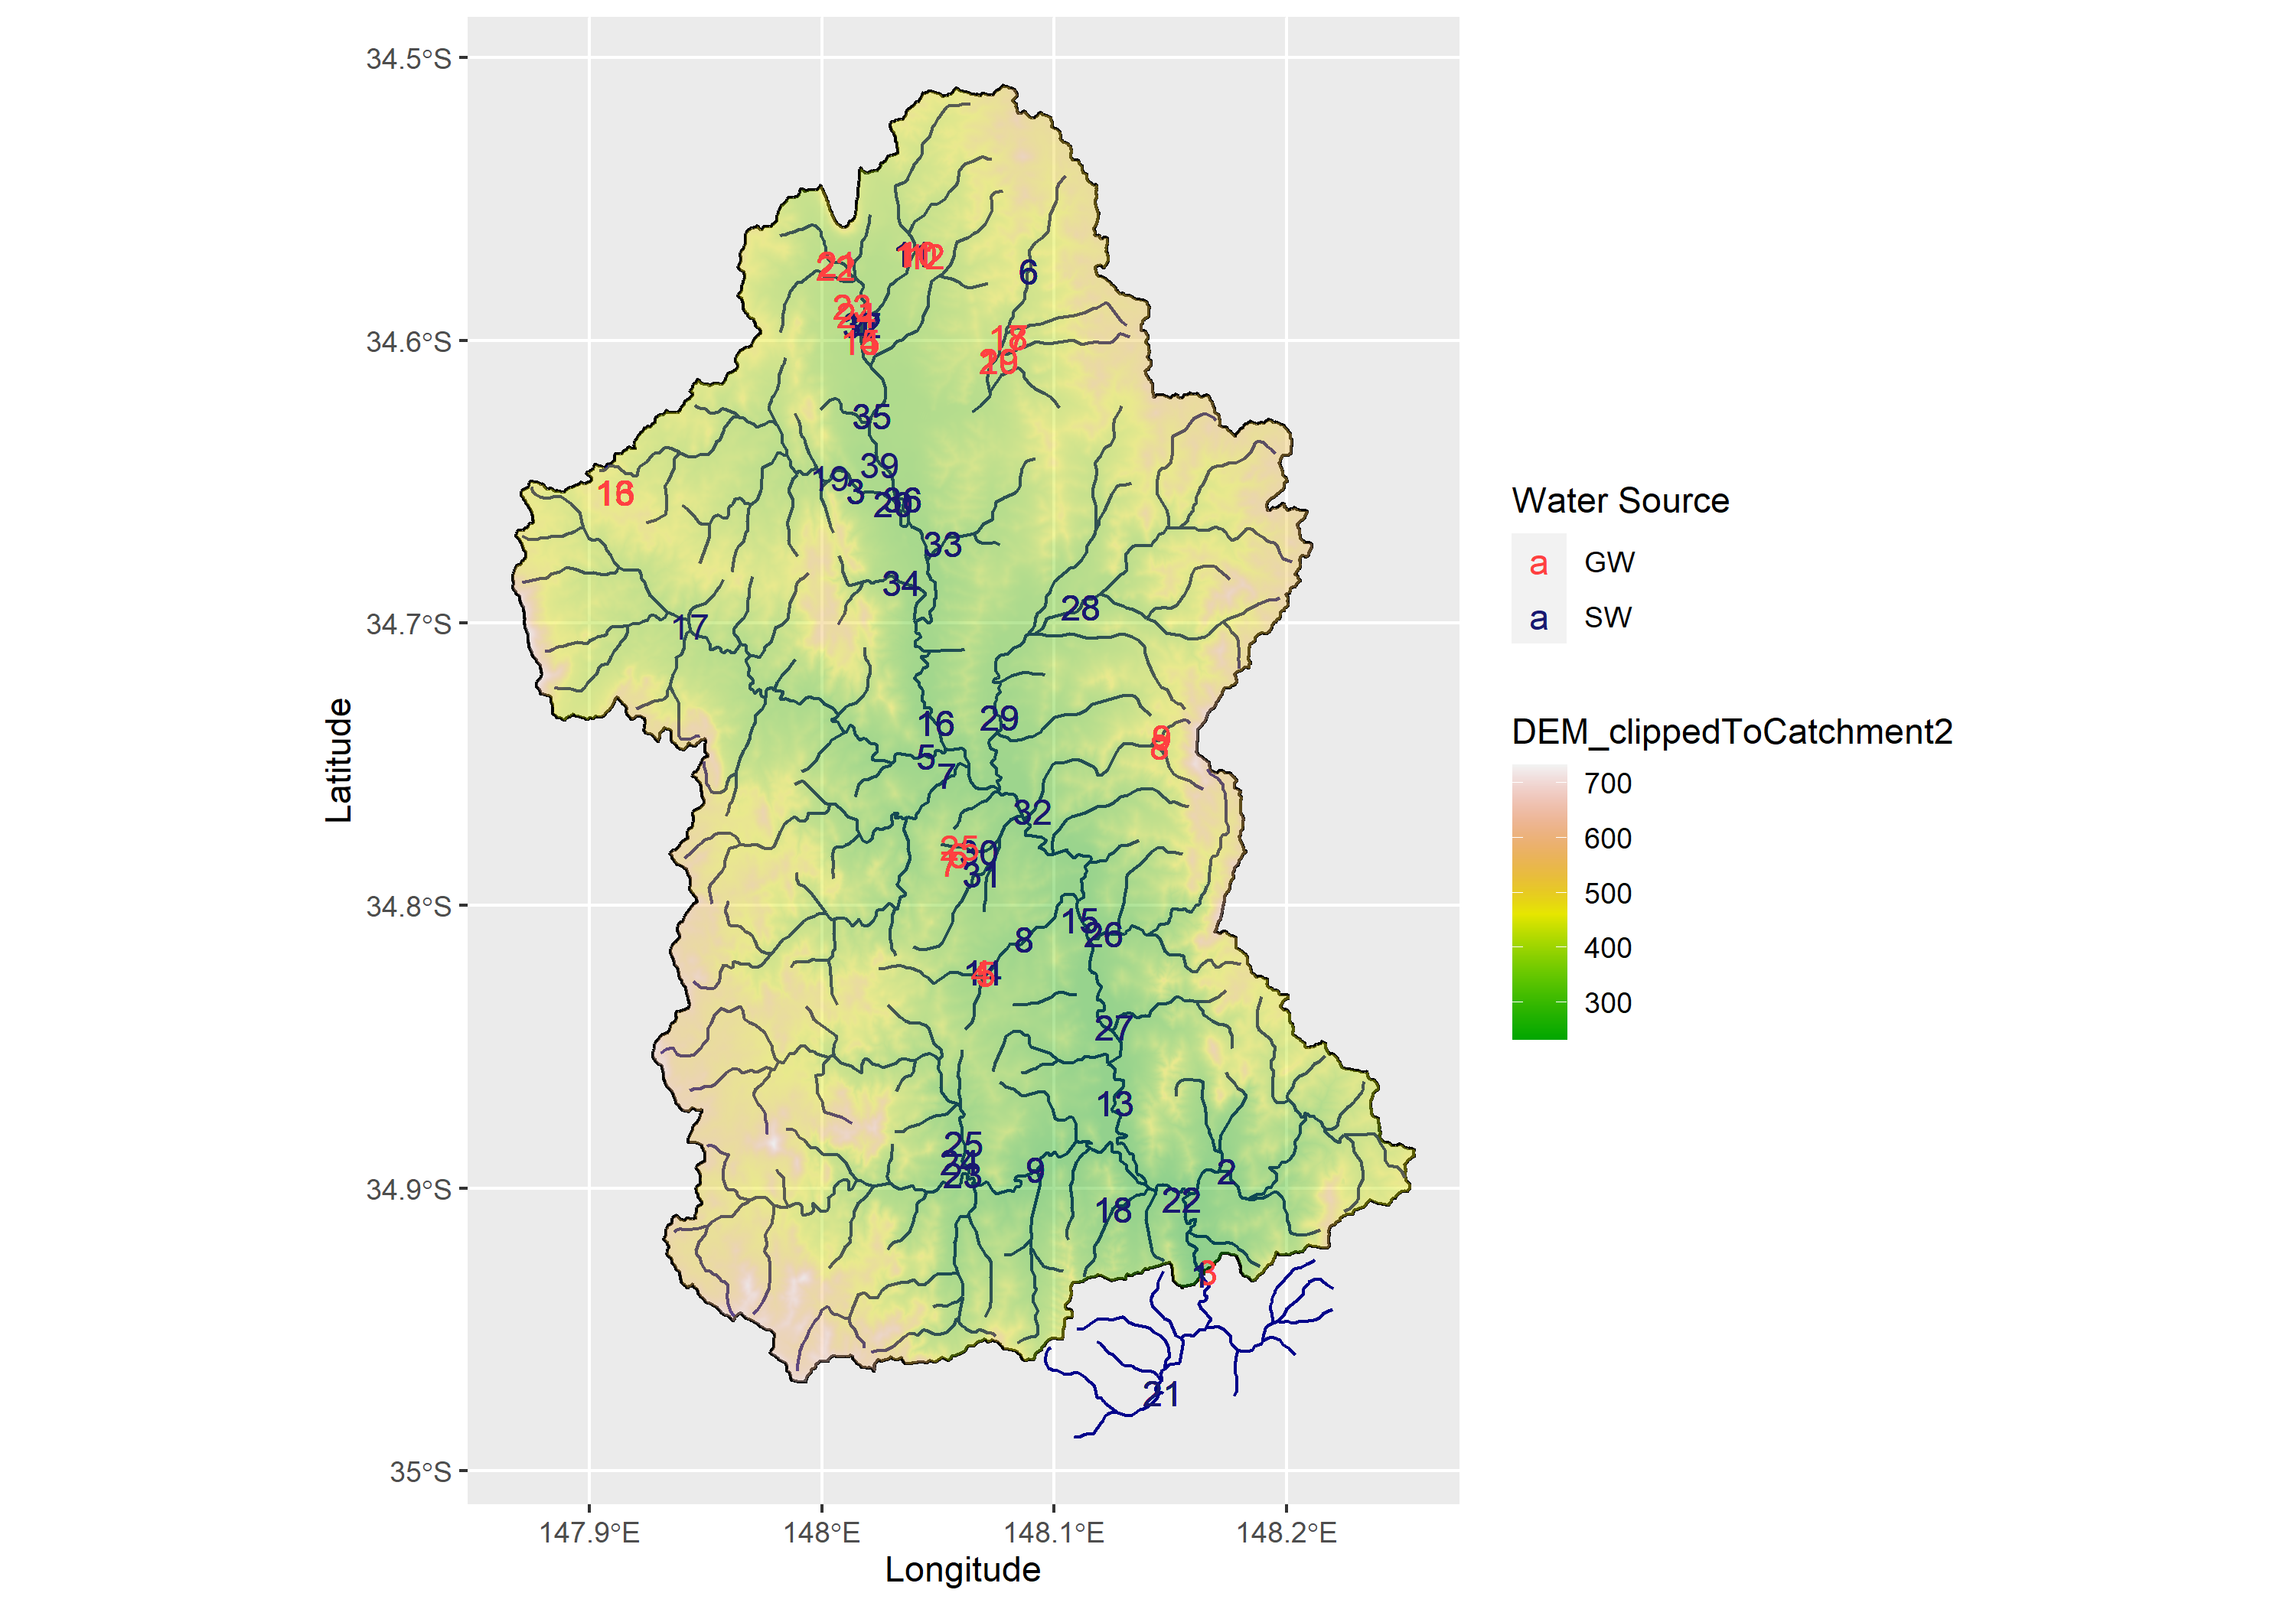
\includegraphics[width=0.8\linewidth]{Figures/gw_or_sw_map} \caption{Muttama Catchment Sampling Locations with Elevation. Symbol colour indicates whether location was a groundwater or surface water source, with blue being surface water and brown/orange being groundwater. The numbers on the map represent the sample location number.}\label{fig:samplemap}
\end{figure}

The depth to the nearest groundwater table varies across the Muttama
catchment and it ranges from \textless{} 2m to 20m below ground level
\citep{DECC2009}. Deep groundwater in the catchment area occurs mostly
in fractured rock aquifers common on the eastern, and western fringes of
the catchment. In contrast shallow groundwater is associated with
unconfined alluvial, colluvial, and eluvial aquifers. Some aquifers in
the northern part of this catchment show artesian behavior
\citep{Webb1999, Akter2018}.

Saline areas of the catchment tend to be associated with geological
heterogeneity, primarily the sedimentary materials in the west and
rhyolite on the northwest side \citep{Conyers2008}. Overall, Muttama
creek is a significant salt contributor to the downstream Murrumbidgee
river with around 58\% from cyclic sources and 42\% salts originating
from mineral weathering \citep{Conyers2008}.

\subsection{Data Collection}

\subsubsection{Data Sources}

The water quality dataset contains data from 4 main sampling sources
related to four distinct groups of ``people'' doing the sample
collection. The term ``people'' is used here loosely, as it mainly
related to four different types of sampling campaigns, which potentially
had differences in the rigour of the sampling campaign (Quality control,
types of samples taken, training of the people taking the samples).
These groups are designated as:

\begin{itemize}
\item
  Source 1: Data from the PhD study by Akter \citeyearpar{Akter2018}.
\item
  Source 2: Data from the sampling campaign of two former students, the
  PhD from Lessels \citeyearpar{Lessels2014} and unpublished data from
  another student, E. Milne.
\item
  Source 3: A dataset collected by undergraduate and postgraduate
  students as part of field trips in different units of study at the
  University of Sydney is identified as ``Student data''. This data was
  sampled ``ad-hoc'' during the field trip period using standard
  sampling protocols as described for the data from Akter
  \citeyearpar{Akter2018}.
\item
  Source 4: Data from several autosamplers installed in the catchment
  during the PhD from Lessels \citeyearpar{Lessels2014}. Because these
  samples were not taken by a ``person'' and were taken on a flow
  weighted basis, we separated the data from the ``grab'' samples in the
  other methods.
\end{itemize}

Overall, 1065 water samples were collected from 62 sample locations over
the 2010 - 2020 period. However, not all sites were sampled at all times
and not all samples were fully analysed for all hydrogeochemical
variables. Both surface water and groundwater samples were collected (23
groundwater sample sites and 39 surface water sites) distributed across
the catchment, depending on standing water availability and access.

In addition to the water quality dataset, data from 23 groundwater data
loggers was downloaded from the same groundwater sample sites as in the
hydrogeochemical dataset.

\subsubsection{Hydrogeochemical Variables}

The overall structure of the hydrogeochemical dataset consists of
repeated measurements over time at multiple locations in Muttama
catchment. For each location the name of the location and the spatial
coordinates were recorded in decimal degrees (Longitude = x and Latitude
= y) as well as whether the location was a groundwater or a surface
water location. The names of the locations are fairly random and basic
locality indicators, which cannot be interpreted exactly.

The data for each location consist of up to six variables which were
measured in the field (Table \ref{tab:TableMeasurements}). These were
complemented by laboratory analysis, which repeated some of the field
measurements, and for an additional 15 anion and cation variables.

\clearpage
\begin{table}

\caption{\label{tab:TableMeasurements}Variables measured in the field and laboratory}
\centering
\begin{tabular}[t]{l|l|l|l}
\hline
Field measurements & Lab repeat & Anions & Cations\\
\hline
pH & pH & NO3 & Na\\
\hline
EC (Electrical conductivity) & EC & NH4 & Ca\\
\hline
SPC (temperature corrected EC) & SPC & NH3 & Mg\\
\hline
Temperature &  & Br & K\\
\hline
Alkalinity (HCO3) &  & PO4 & S\\
\hline
Dissolved Oxygen (DO) &  & SO4 & P\\
\hline
Turbidity &  &  & Al\\
\hline
 &  &  & Fe\\
\hline
 &  &  & Si\\
\hline
\end{tabular}
\end{table}

The variables pH, EC, SPC, Temperature, and in some cases DO and
Turbidity were measured using a range of field probes. All field probes
measured pH, EC, Temperature and calculated SPC. Early measurements used
a YSI probe that included a turbidity and DO probe (YSI 6600 and YSI 600
for surface and groundwater, respectively). Later groundwater samples
used a different YSI probe (YSI ProPlus multi-parameter) that only
included a DO probe. Later surface water and groundwater sampling used a
Xylem EXO probe which also included DO and turbidity.

Anions in most of the samples were analysed using high-performance
liquid chromatography method (Dionex P680 HPLC) and cations were
measured on acidified samples using an Inductively Coupled Plasma
Optical Emission Spectrometer (ICP-OES, Varian 720-ES) at the University
of Sydney \citep{Akter2018}. Duplicate samples in the analysis had a
reported relative percentage difference (RPD) lower than 5\% in part of
the sample dataset \citep{Akter2018}. Some of the samples in the
undergraduate student sample set (Source 3) were analysed by a
commercial laboratory
(\href{https://www.alsglobal.com/en/locations/asia-pacific/pacific/australia/nsw/sydney-woodpark-environmental}{ALS
Environmental, Smithfield, NSW}). Alkalinity concentrations were
measured in the field within 24h of collection using a HACH digital
titrator (model 16900) \citep{Akter2018}.

Using the cation and anion data, ion balances were calculated from
samples which had a complete set of anion and cation measurements.

\subsection{Continuous variables}

The logger data, which collected groundwater pressure levels at 15 min
and later at 2 hour intervals, were adjusted for the length of the cable
and the height of the standpipe above the ground level. They were
subsequently summarised to raw daily values using an R script
(\texttt{SummariseDailyData.R}), which is stored on the github
repository.

The loggers in the field were uncalibrated. Due to logger failures, gaps
occur in the daily data, followed by replacement of the faulty loggers.
In some cases the cable length was adjusted and this was recorded in the
field notes. Overall, this resulted in data with gaps and sometimes odd
shifts in the recorded data.

Manual water level measurements were taken at each manual sampling date
for hydrogeochemical data.

To correct the groundwater logger data, the daily data was matched to
the observed data using linear regression if more than 3 manual observed
data were available and slope and intercept of the regression had a
p-value \textgreater{} 0.1. If there were less than 3 manual observed
data point for the specific logger an adjustment to the data was based
on the difference between the average observed data and the average
recorded water levels. Otherwise no adjustment was made. This is
slightly tricky: when the manual observations are made, the well is also
purged and the logger is removed from the well. This data (during the
purging and recovery) is removed from the logger data series. As a
result, there is no direct match between the logger data series and the
manual observations.

To explain this more clearly the following pseudo code describes the
process:

\begin{itemize}
\tightlist
\item
  Split the logger data for each ground water well by serial number;
\item
  Interpolate the manual observed values using \texttt{na.approx()} to
  account for the fact that no logger data exists when manual
  measurements are made:
\item
  if there are sufficient observed points (assumed to be \textgreater{}
  3):

  \begin{itemize}
  \tightlist
  \item
    run a regression between interpolated depth and observed depth;
  \item
    check the p-values of the slope and intercept;
  \item
    if the slope is not significant (using p \textgreater{} 0.10):

    \begin{itemize}
    \tightlist
    \item
      use only the intercept to correct the logger data;
    \end{itemize}
  \item
    else

    \begin{itemize}
    \tightlist
    \item
      if the intercept is not signficant, but the slope is:

      \begin{itemize}
      \tightlist
      \item
        use only the slope to correct the logger data;
      \end{itemize}
    \item
      else

      \begin{itemize}
      \tightlist
      \item
        use both slope and intercept of the regression to correct the
        logger data;
      \end{itemize}
    \item
      end if
    \end{itemize}
  \item
    end if
  \end{itemize}
\item
  else

  \begin{itemize}
  \tightlist
  \item
    There are not enough values for a regression, use mean difference
    between logged and observed value to correct the logger data
  \end{itemize}
\item
  end if
\end{itemize}

The code used to match the manually observed data with the logger data
is in the \texttt{Match\_obs\_logger\_data.R}, which is stored in the
github repository associated with this paper.

After the automated process, two of the groundwater level data series
still had substantial discrepancies in some sections of the data. This
was most likely due to the a lack of observed data for the specific
logger. A final manual correction was applied. As this process is based
on judgement of the data by the authors, we documented this in detail in
Appendix 1.

The final corrected data includes a column which describes whether the
data is based on the automatic correction or a further manual
correction.

\subsection{Boxplots and maps}

Using the most complete data, boxplots and spatial maps were generated
to highlight the spatial and temporal variation in the data set. As this
paper is mainly focused on describing the dataset, we chose to use
boxplots to visually highlight statistical differences between data
variables rather than using full statistical analysis.

The mean concentration and interquartile range (25th - 75th percentile)
of the concentration data distributions were calculated to give an
indication of variance of the data in the spatial maps.

All graphs and maps were produced using R \citep{R2022}. All code can be
found in the associated github repository

\section{Results}

\subsection{Distribution of missing Values}

\clearpage
\begin{figure}
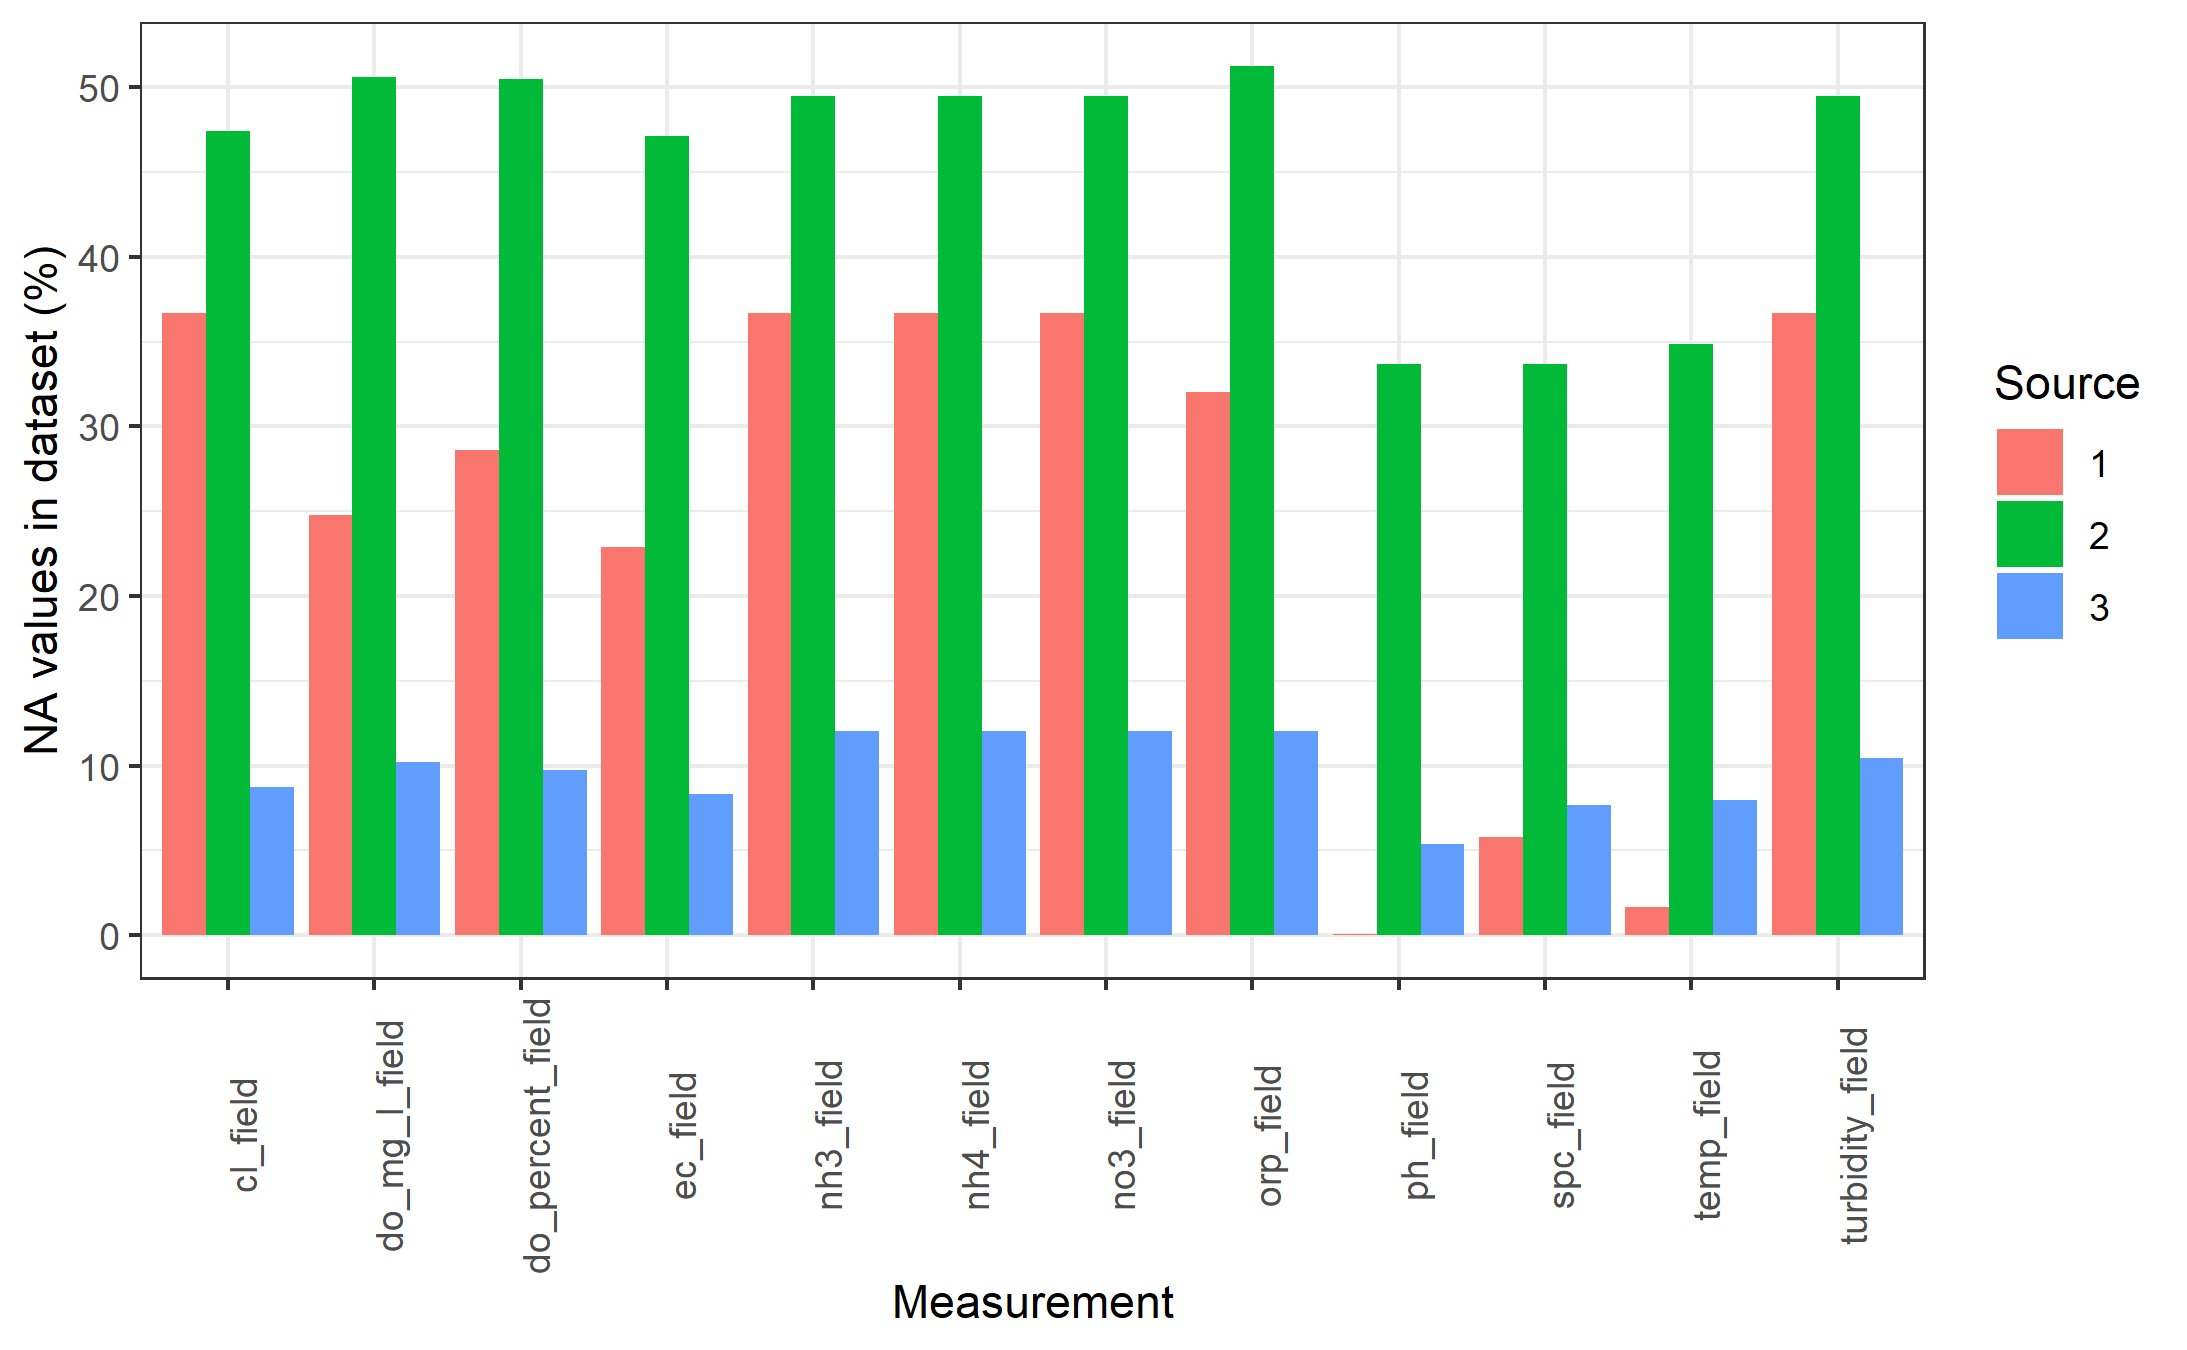
\includegraphics[width=0.9\linewidth]{Figures/na_count} \caption{Distribution of missing values for the different data sources and measurement types.}\label{fig:na-plot}
\end{figure}

\begin{figure}
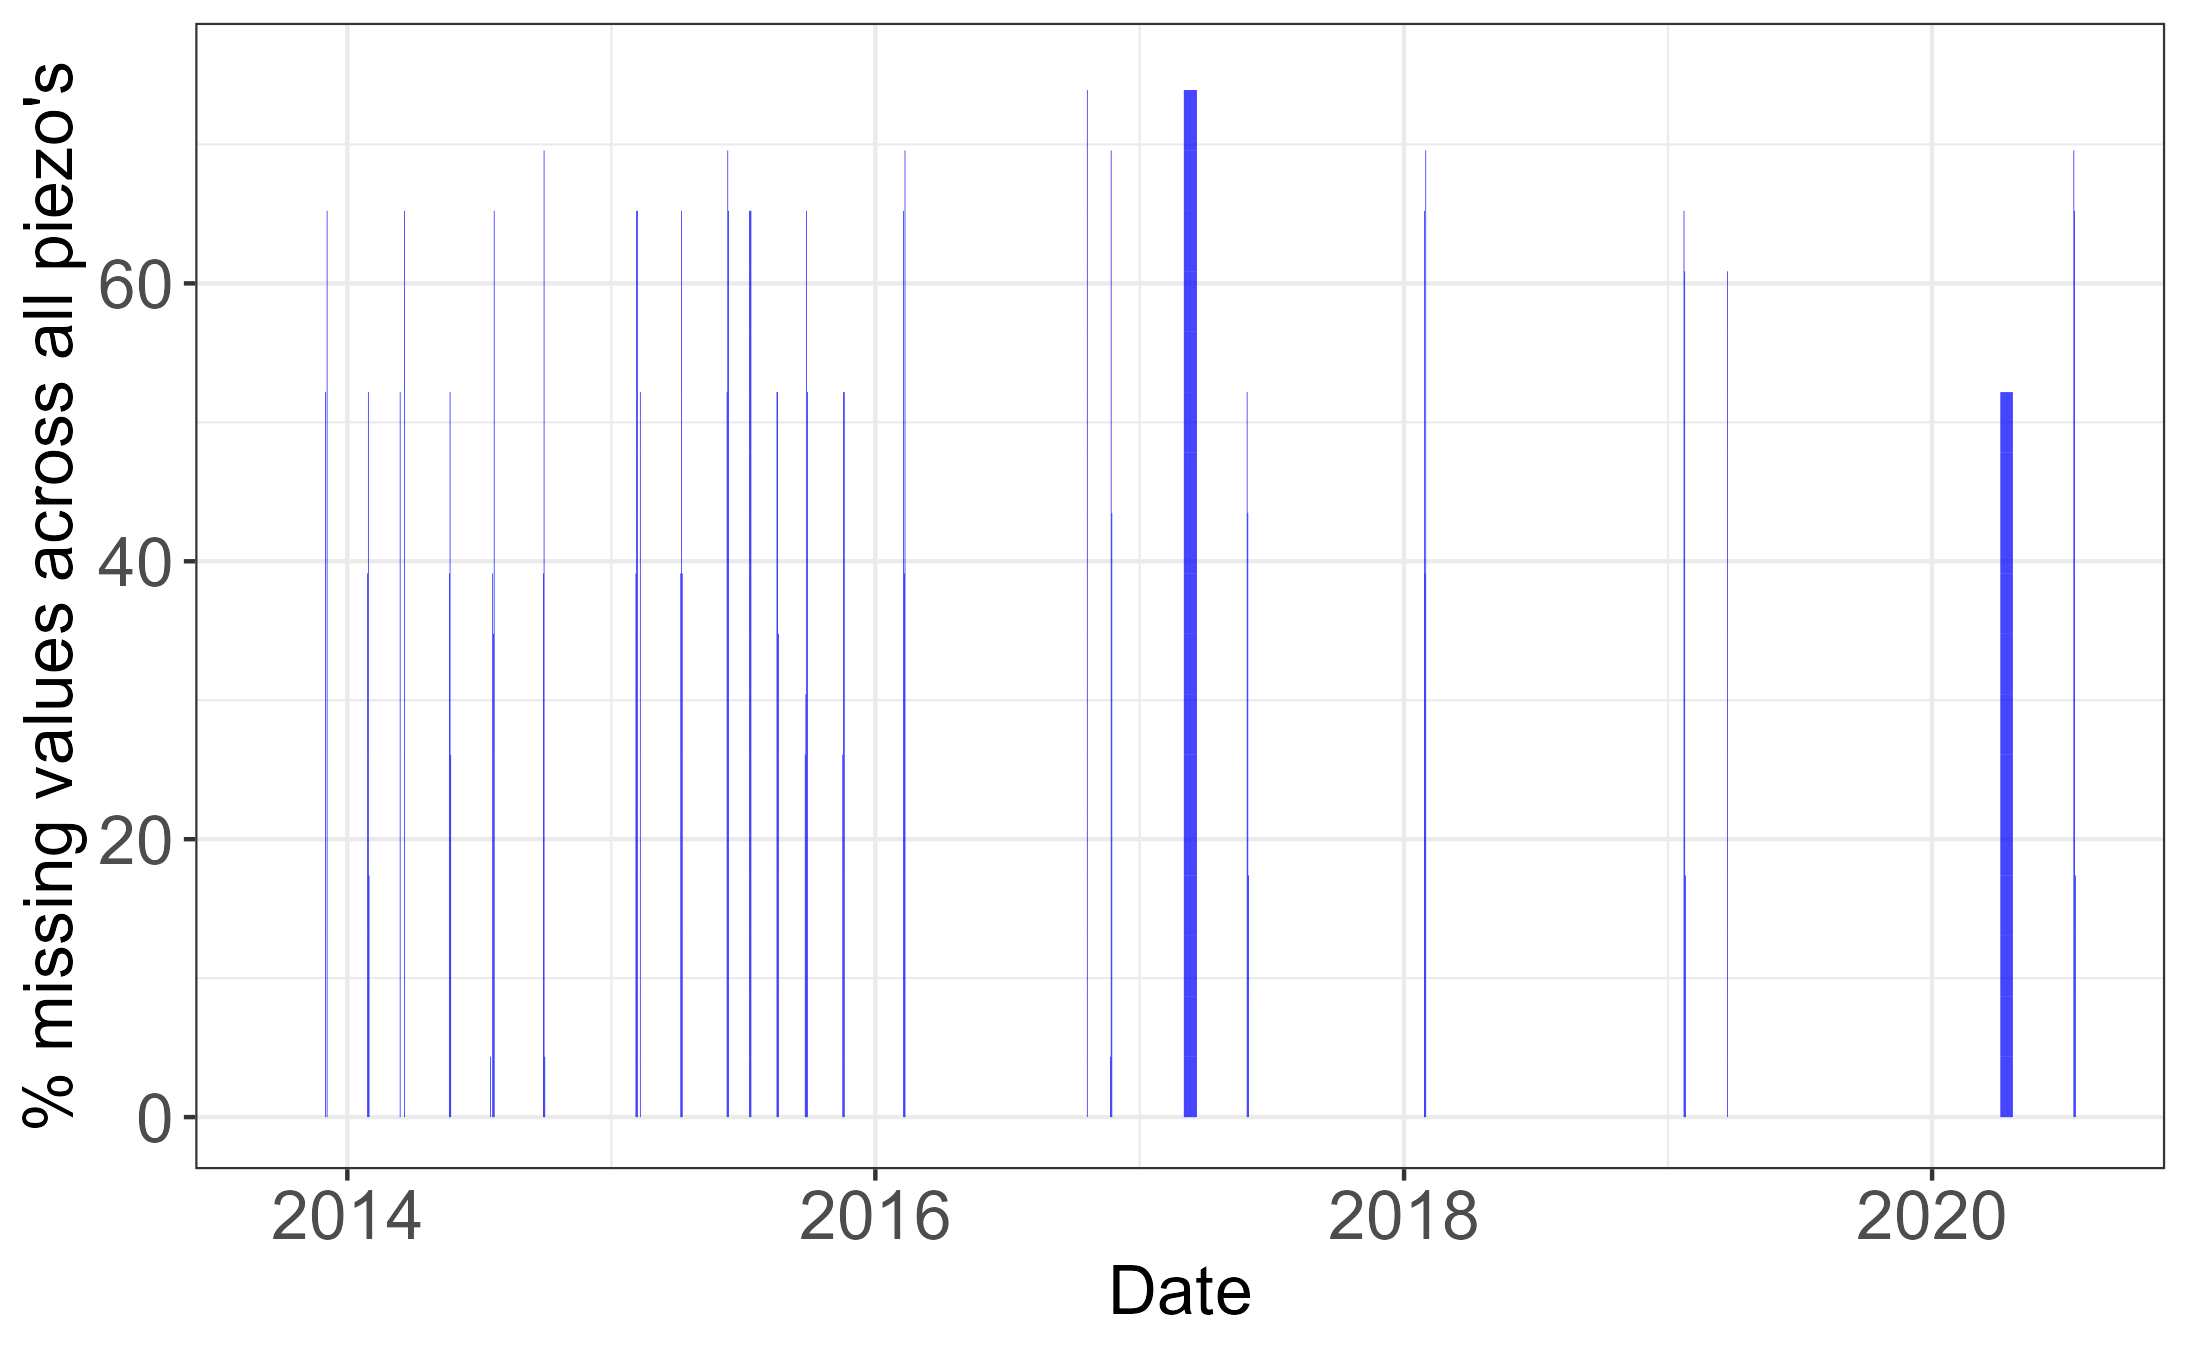
\includegraphics[width=0.9\linewidth]{Figures/na_GW} \caption{Percent missing values for the groundwater data across all piezometers.}\label{fig:gw-na-plot}
\end{figure}

In the hydrogeochemistry data, data source 3 was the most complete in
terms of variables analysed, because in this set more variables were
analysed in the commercial lab (Fig \ref{fig:na-plot}). Some of the
variables analysed in the commercial lab were not analysed with the
equipment at the University of Sydney. However, source 3 had the
smallest number of overall samples. Source 2 has the most incomplete
data points. Source 4 has a very consistent number of missing values,
possibly because not all samples were analysed in the set. For source 2,
the missing data suggests that for many of the samples only a few of the
variables were measured and analysed as highlighted above. In the data
from source 2, almost 50\% of samples are incomplete in terms of the
measurement of all the variables in Table 2. Similarly, source 1 had
more incomplete data, because some of the minor elements were not
analysed. The field recorded variables pH, EC, SPC and Temperature were
the most complete as they were generally measured directly in the field.
Analysis of bicarbonate in the field only started around 2014. Thus the
distribution of the NA values in the overall dataset is mostly a
reflection of the time period of sampling and the change in methodology
over the ten years of sampling.

In the groundwater level time series, the missing data relate mostly to
the logger failures and the different times that wells were
instrumented. Rather than giving a full breakdown by well location, the
overall level of completeness of the series is displayed (Fig
\ref{fig:gw-na-plot}).

\subsubsection{Groundwater compared with Surface water}

\clearpage
\begin{table}

\caption{\label{tab:TableElementstats}Summary statistics for elements measured in the field}
\centering
\begin{tabular}[t]{l|r|r|r|r|r|r}
\hline
\multicolumn{1}{c|}{} & \multicolumn{3}{c|}{GW} & \multicolumn{3}{c}{SW} \\
\cline{2-4} \cline{5-7}
Element & Mean & Min & Max & Mean & Min & Max\\
\hline
temp\_field & 17.4 & 11.4 & 30.8 & 15.0 & 4.1 & 32.9\\
\hline
do\_percent\_field & 19.9 & -3.2 & 70.7 & 87.9 & 29.8 & 184.0\\
\hline
do\_mg\_l\_field & 1.9 & 0.0 & 6.7 & 7.7 & 2.2 & 18.3\\
\hline
spc\_field & 4589.6 & 347.4 & 14317.0 & 1053.3 & 61.0 & 4354.0\\
\hline
ec\_field & 3821.8 & 457.0 & 11029.2 & 1371.5 & 117.0 & 4163.0\\
\hline
ph\_field & 7.3 & 6.3 & 8.8 & 8.0 & 6.7 & 10.0\\
\hline
orp\_field & 26.6 & -328.1 & 242.0 & 78.2 & -126.5 & 211.1\\
\hline
turbidity\_field &  & Inf & -Inf & 14.0 & 0.5 & 44.0\\
\hline
cl\_field & 320.0 & 320.0 & 320.0 & 602.8 & 30.0 & 3830.0\\
\hline
no3\_field &  & Inf & -Inf & 3.7 & 1.5 & 6.5\\
\hline
nh4\_field &  & Inf & -Inf & 1.3 & 0.1 & 7.5\\
\hline
nh3\_field &  & Inf & -Inf & 0.0 & 0.0 & 0.5\\
\hline
\end{tabular}
\end{table}

Groundwater samples have quite a distinctive signature compared to the
surface water samples (Fig \ref{fig:gw_sw-plot}). For example,
groundwater samples tend to be higher in EC and lower in pH compared to
surface water samples. Since `Source 1' collected most of the
groundwater samples, this results in differences between data collection
sources. Field SPC measurements were used to represent EC since these
samples had the best coverage.

\clearpage

\begin{figure}
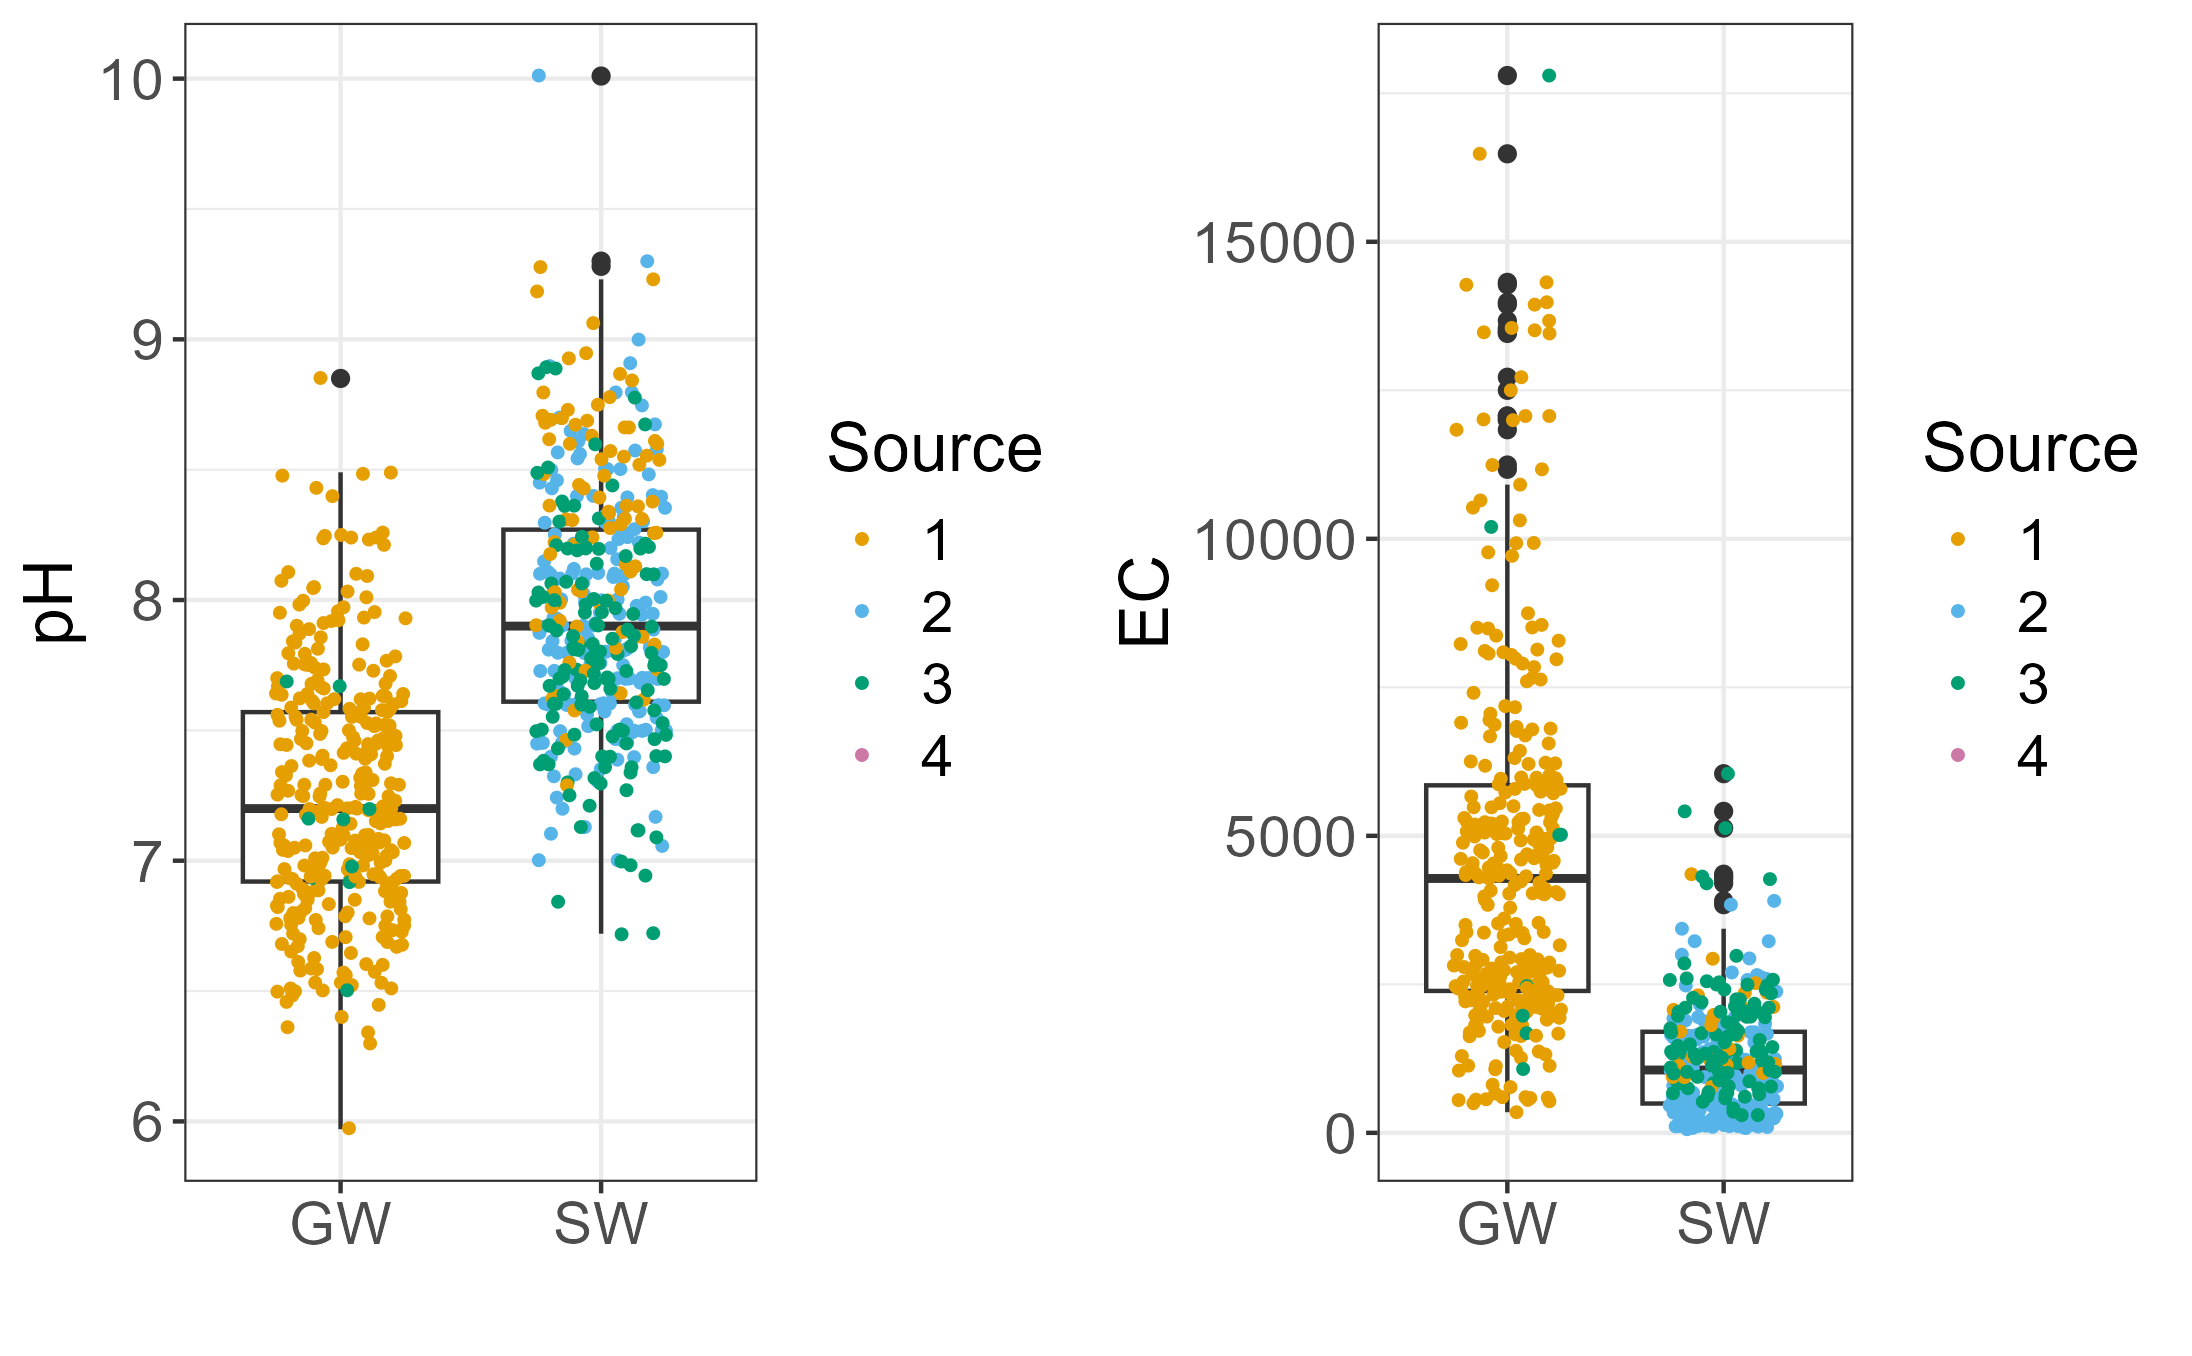
\includegraphics[width=0.8\linewidth]{Figures/gwsw} \caption{Difference in pH and EC for groundwater and surface water samples. The source of the data (the samping group) is indicated with colour}\label{fig:gw_sw-plot}
\end{figure}

\subsection{Temporal Distribution of Data}

\clearpage

\begin{figure}
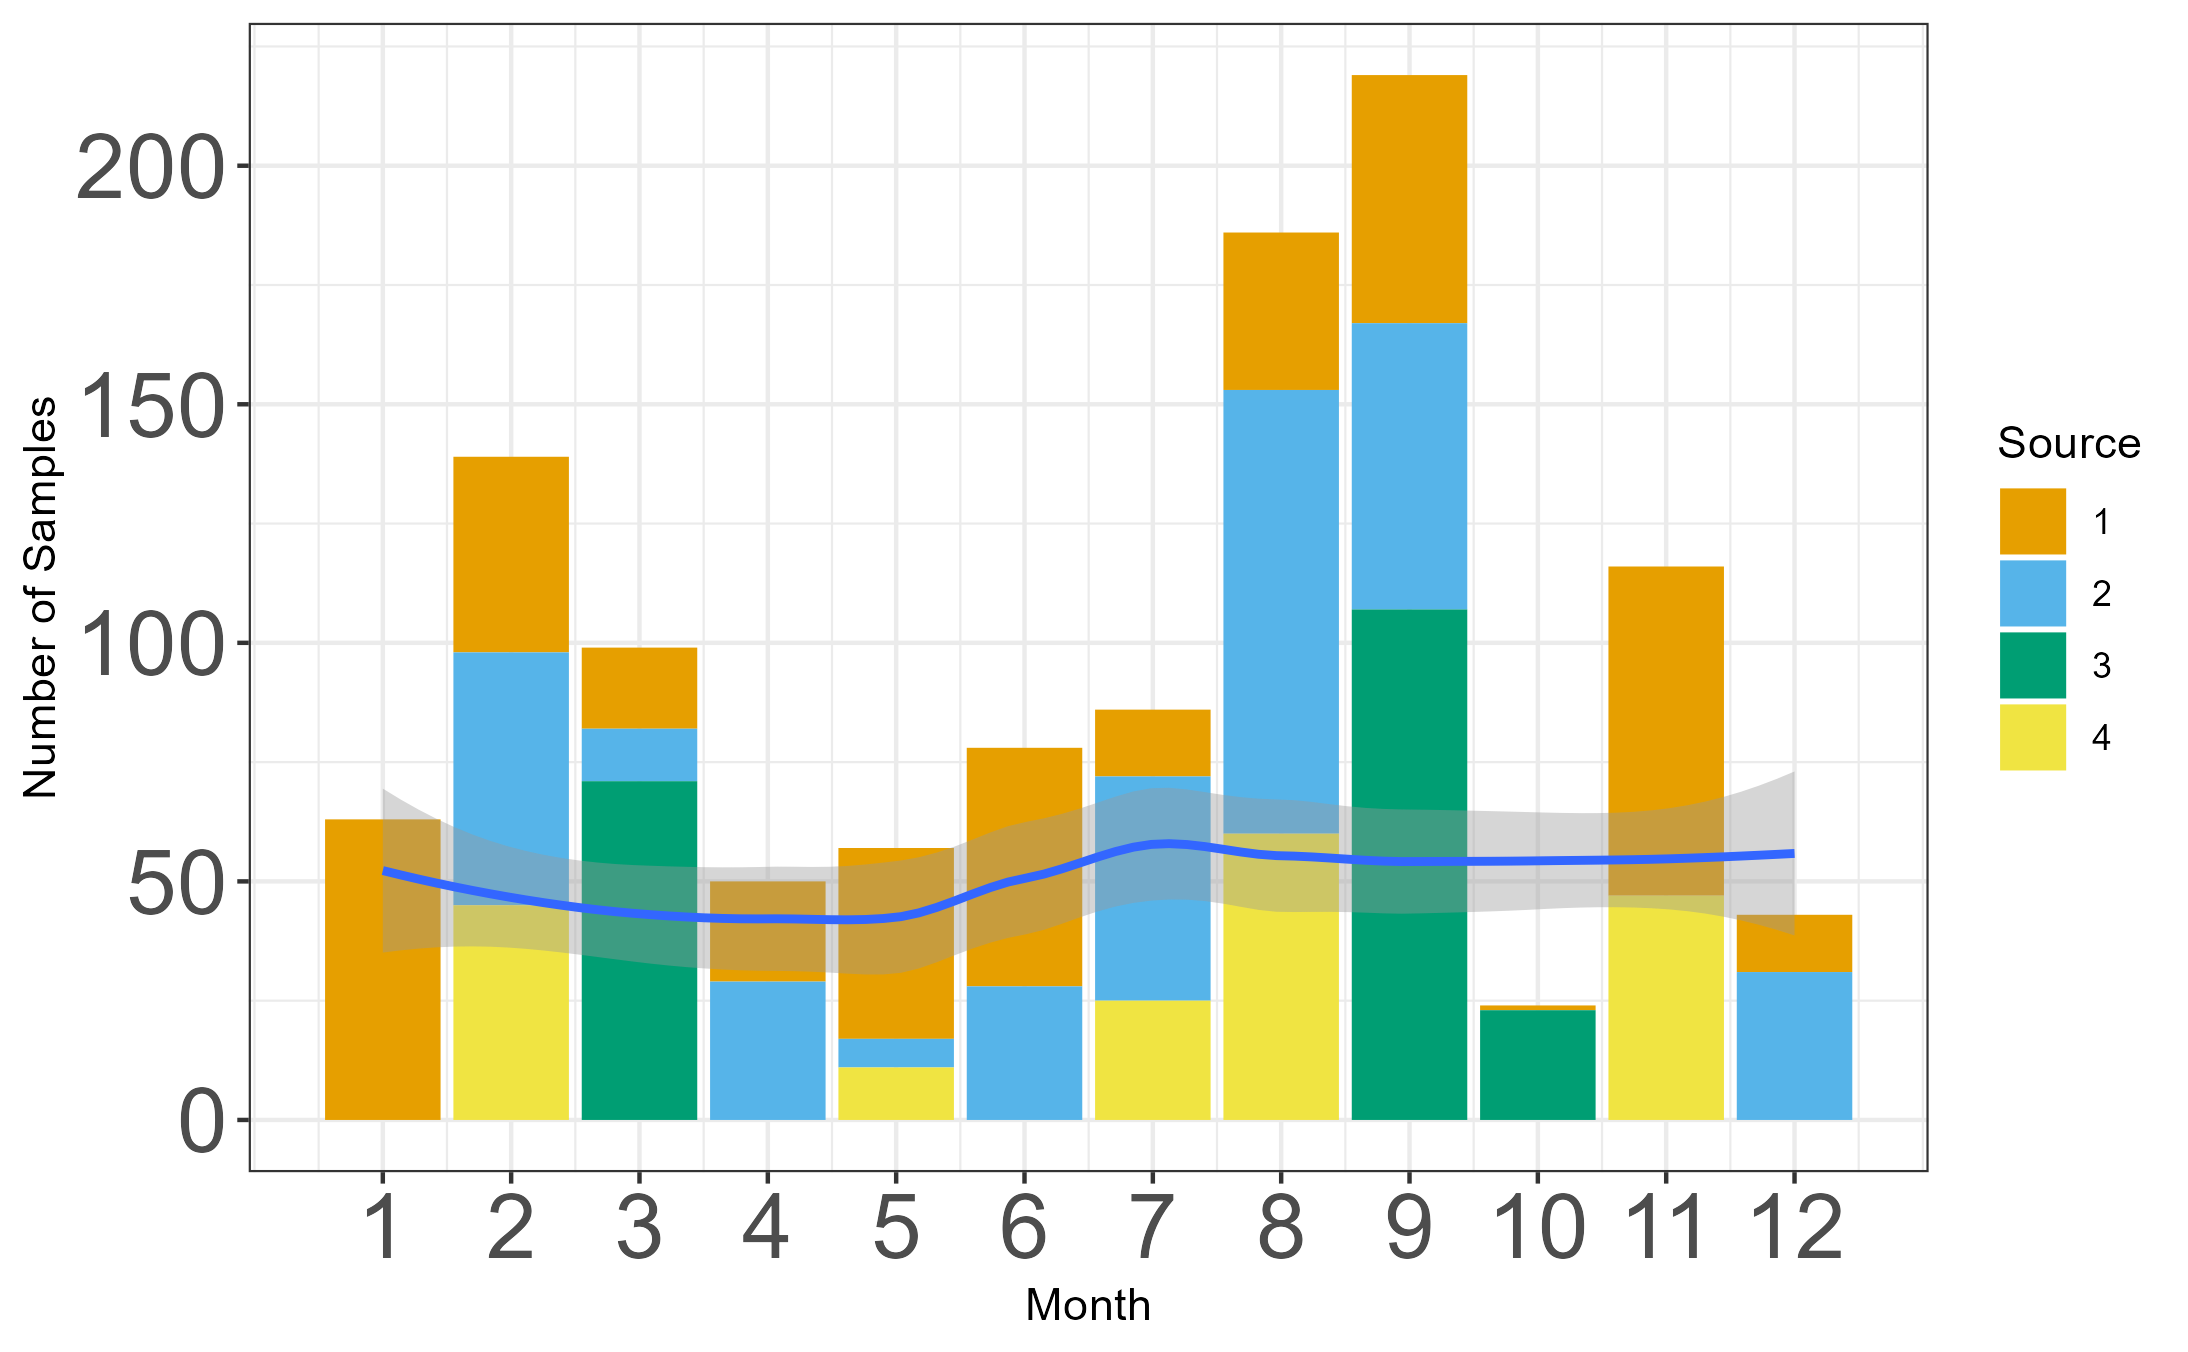
\includegraphics[width=0.5\linewidth]{Figures/monthly} \caption{Distribution of samples throughout the year (total number of samples collected during each month) against average monthly rainfall during the study period. }\label{fig:month-plot}
\end{figure}

Overall the water quality sampling appears to have a reasonable
distribution across all months (Fig \ref{fig:month-plot}), so seasonal
trends should be identifiable in the data. Average rainfall data (1995 -
2022) does not indicate any major seasonal trends, although there is a
slight dominance of rainfall in early Austral Spring (months 9 and 10,
September and October). This also explains the higher number of samples
because, we would organise more sampling trips in this period, and
spatially more channels could be sampled for surface water. The timing
of Source 3, (the student data) is a clear effect of yearly field trips,
which tended to occur at approximately the same time of the year in late
September/early October.

\clearpage

\begin{figure}
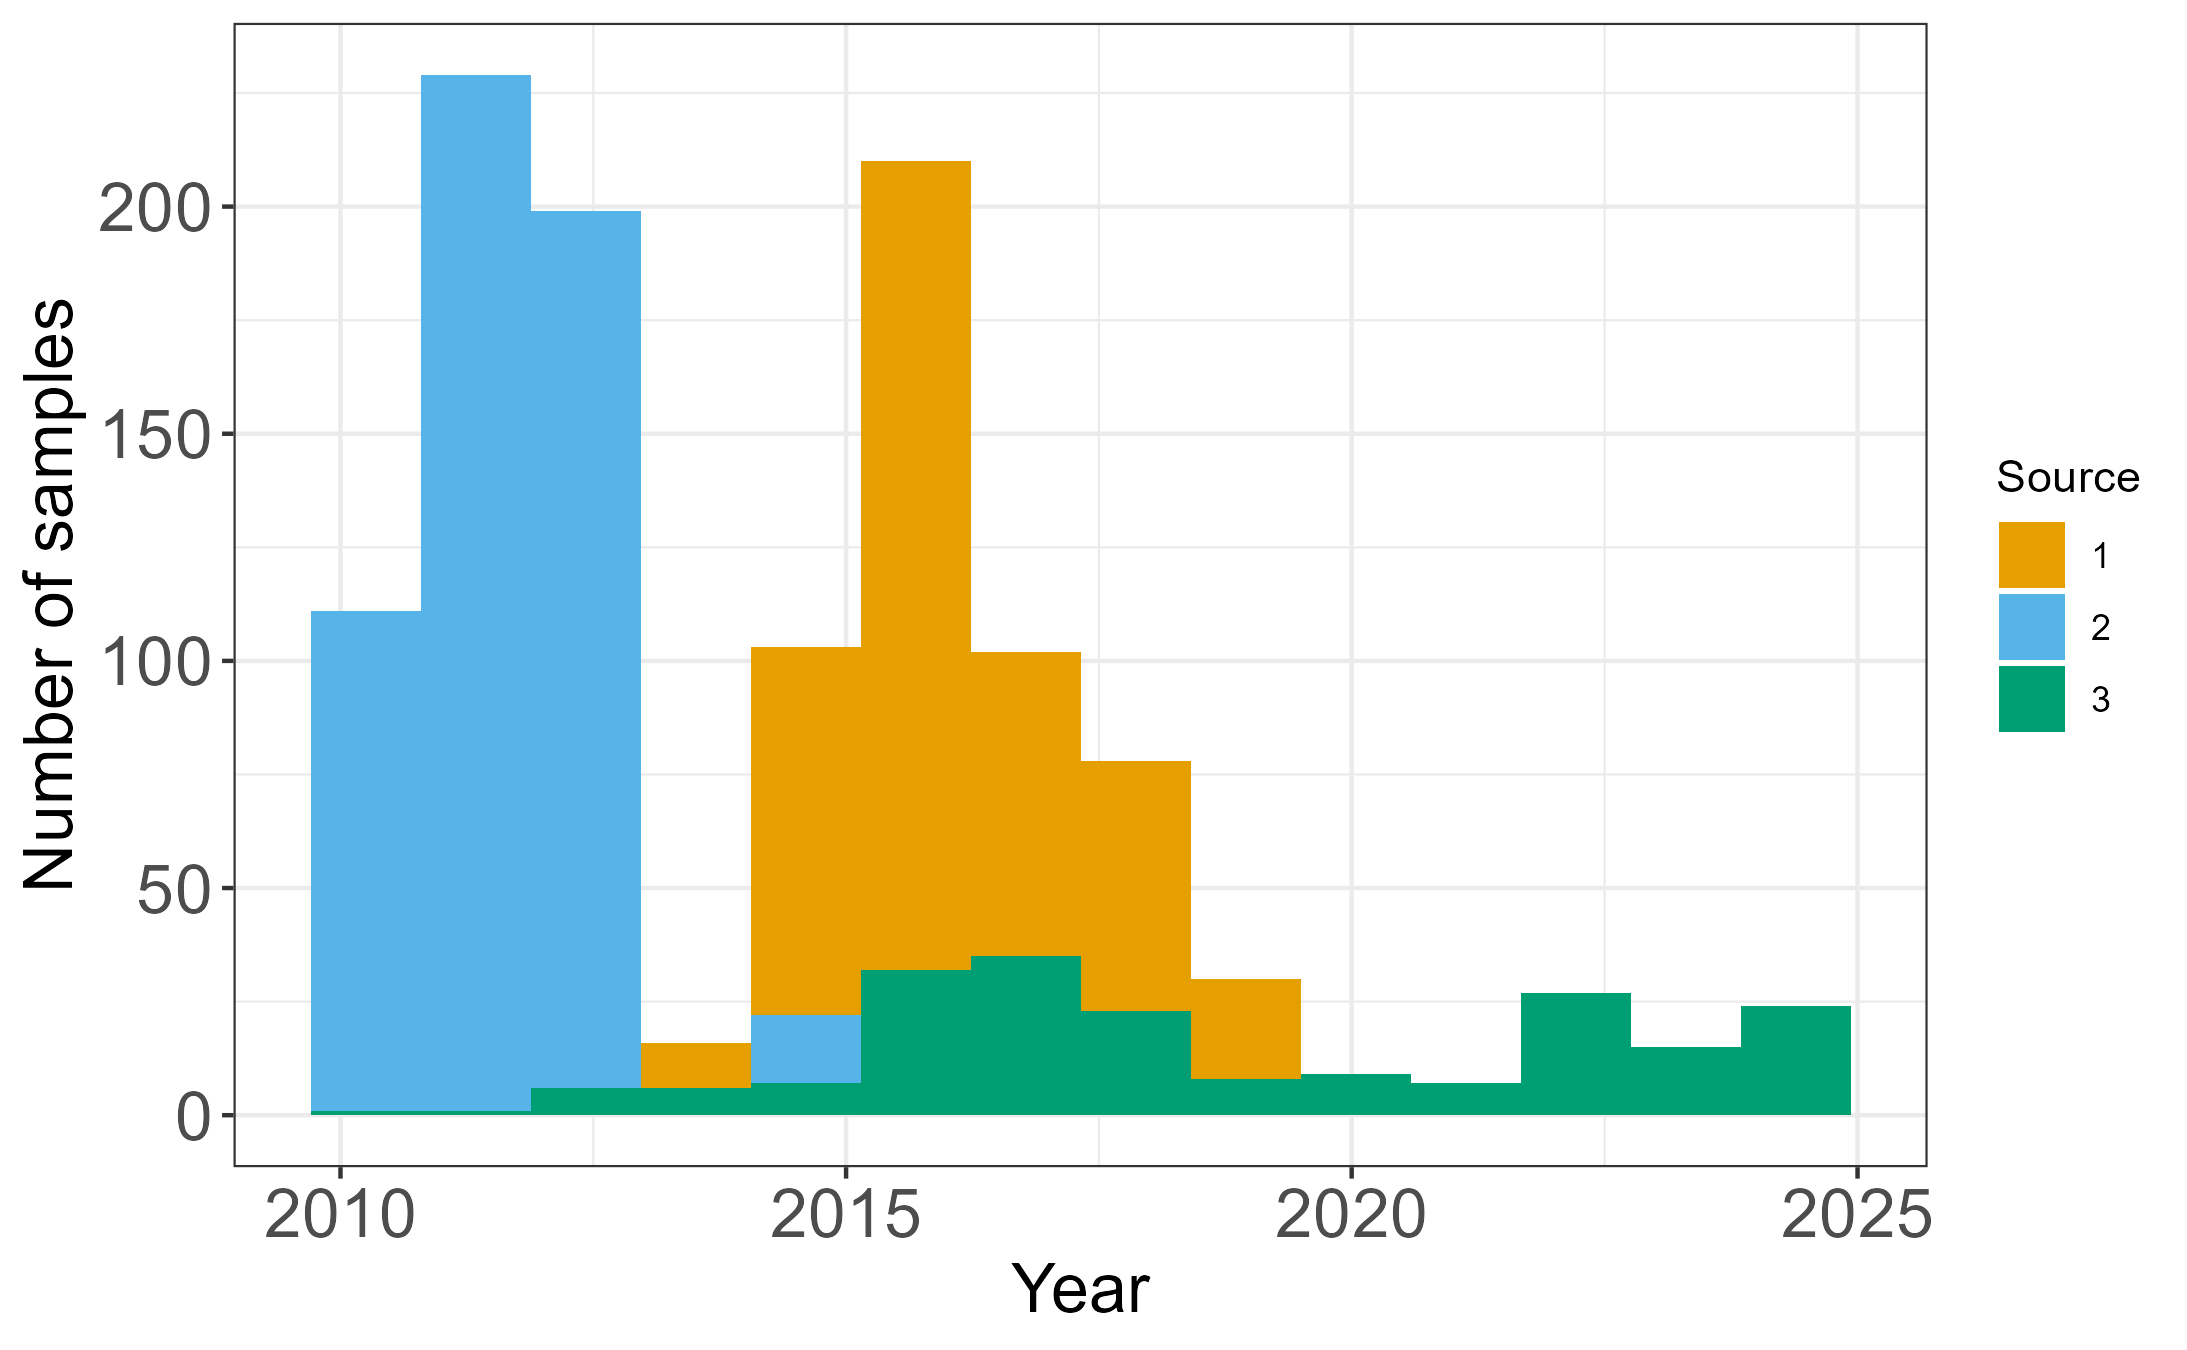
\includegraphics[width=0.5\linewidth]{Figures/annual} \caption{Distribution of samples over the study period (total number of samples collected during each year) against average monthly rainfall during the study period. }\label{fig:annual-plot}
\end{figure}

The number of samples collected in each year relative to the different
sources changes throughout the years reflecting the duration of the
different studies and funding cycles (Fig \ref{fig:annual-plot});
however the data is still well-distributed enough that overall trends
should be clear. In addition, some of the sample volumes can be related
to the occurrence of rainfall, as in drier years several of the channels
would be dry and no sampling of surface water could occur.

Consistent groundwater sampling commenced later in the project, which
means that there are very few groundwater samples before 2013. In
contrast, the autosamplers were installed early in the project and there
are no samples from this source after 2013.

\clearpage

\begin{figure}
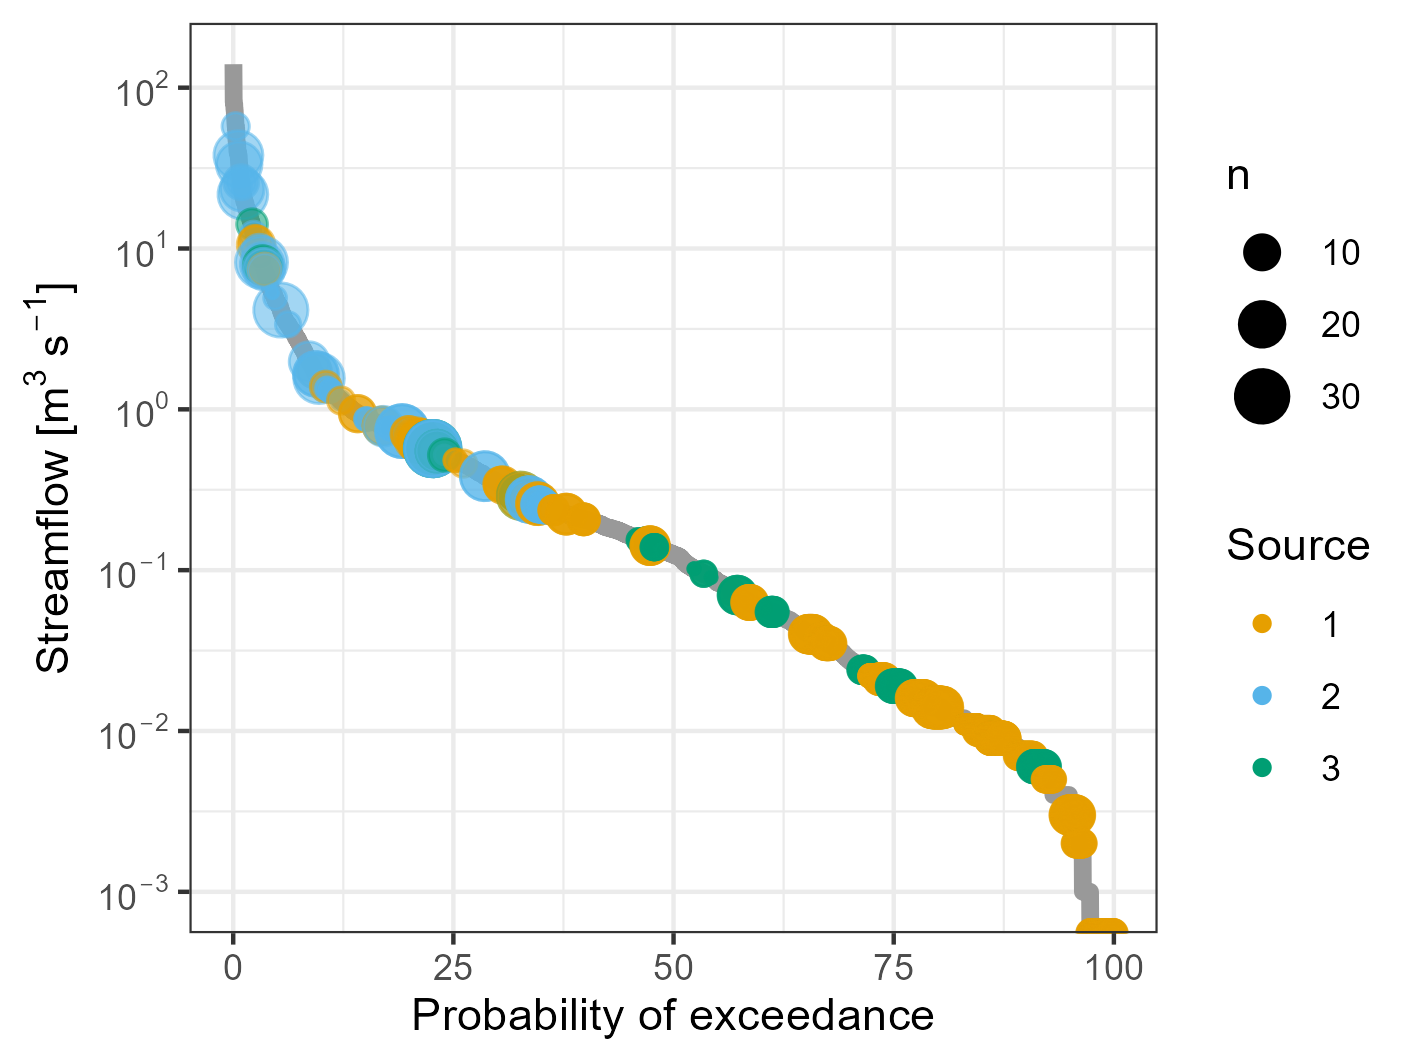
\includegraphics[width=0.8\linewidth]{Figures/FDC} \caption{Sample distribution on flow duration curve derived from flow data from Coolac autosampler.}\label{fig:FDC}
\end{figure}

Surface water samples were reasonably well distributed across the flow
duration curve, with only a possible bias towards periods of medium
flow. This is most likely since many of the surface water sampling
points are often completely dry during periods of low flow, and
therefore cannot be sampled. Conversely, there are no manual samples
during high or very high flow as during flood situations sampling was
dangerous and restricted by work health and safety considerations. The
samples at high flow are all from our automated sampling.

\clearpage
\begin{figure}
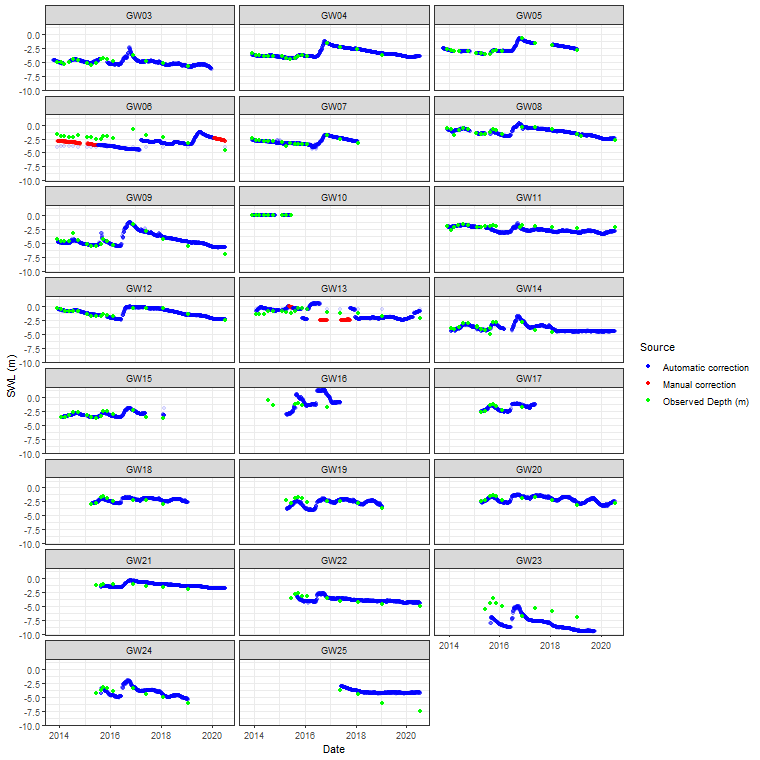
\includegraphics[width=1\linewidth]{Figures/Final_Corrected_piezodepths} \caption{Overview of the corrected groundwater time series for all the wells}\label{fig:gw-series}
\end{figure}

The overall corrected groundwater timeseries shows the shorter time that
loggers were installed in the wells (\ref{fig:gw-series}). It also
indicates that the manual data is not always fully matched with the
logger data, but further corrections are likely to be speculation.

\subsection{Spatial variation}

\clearpage
\begin{figure}
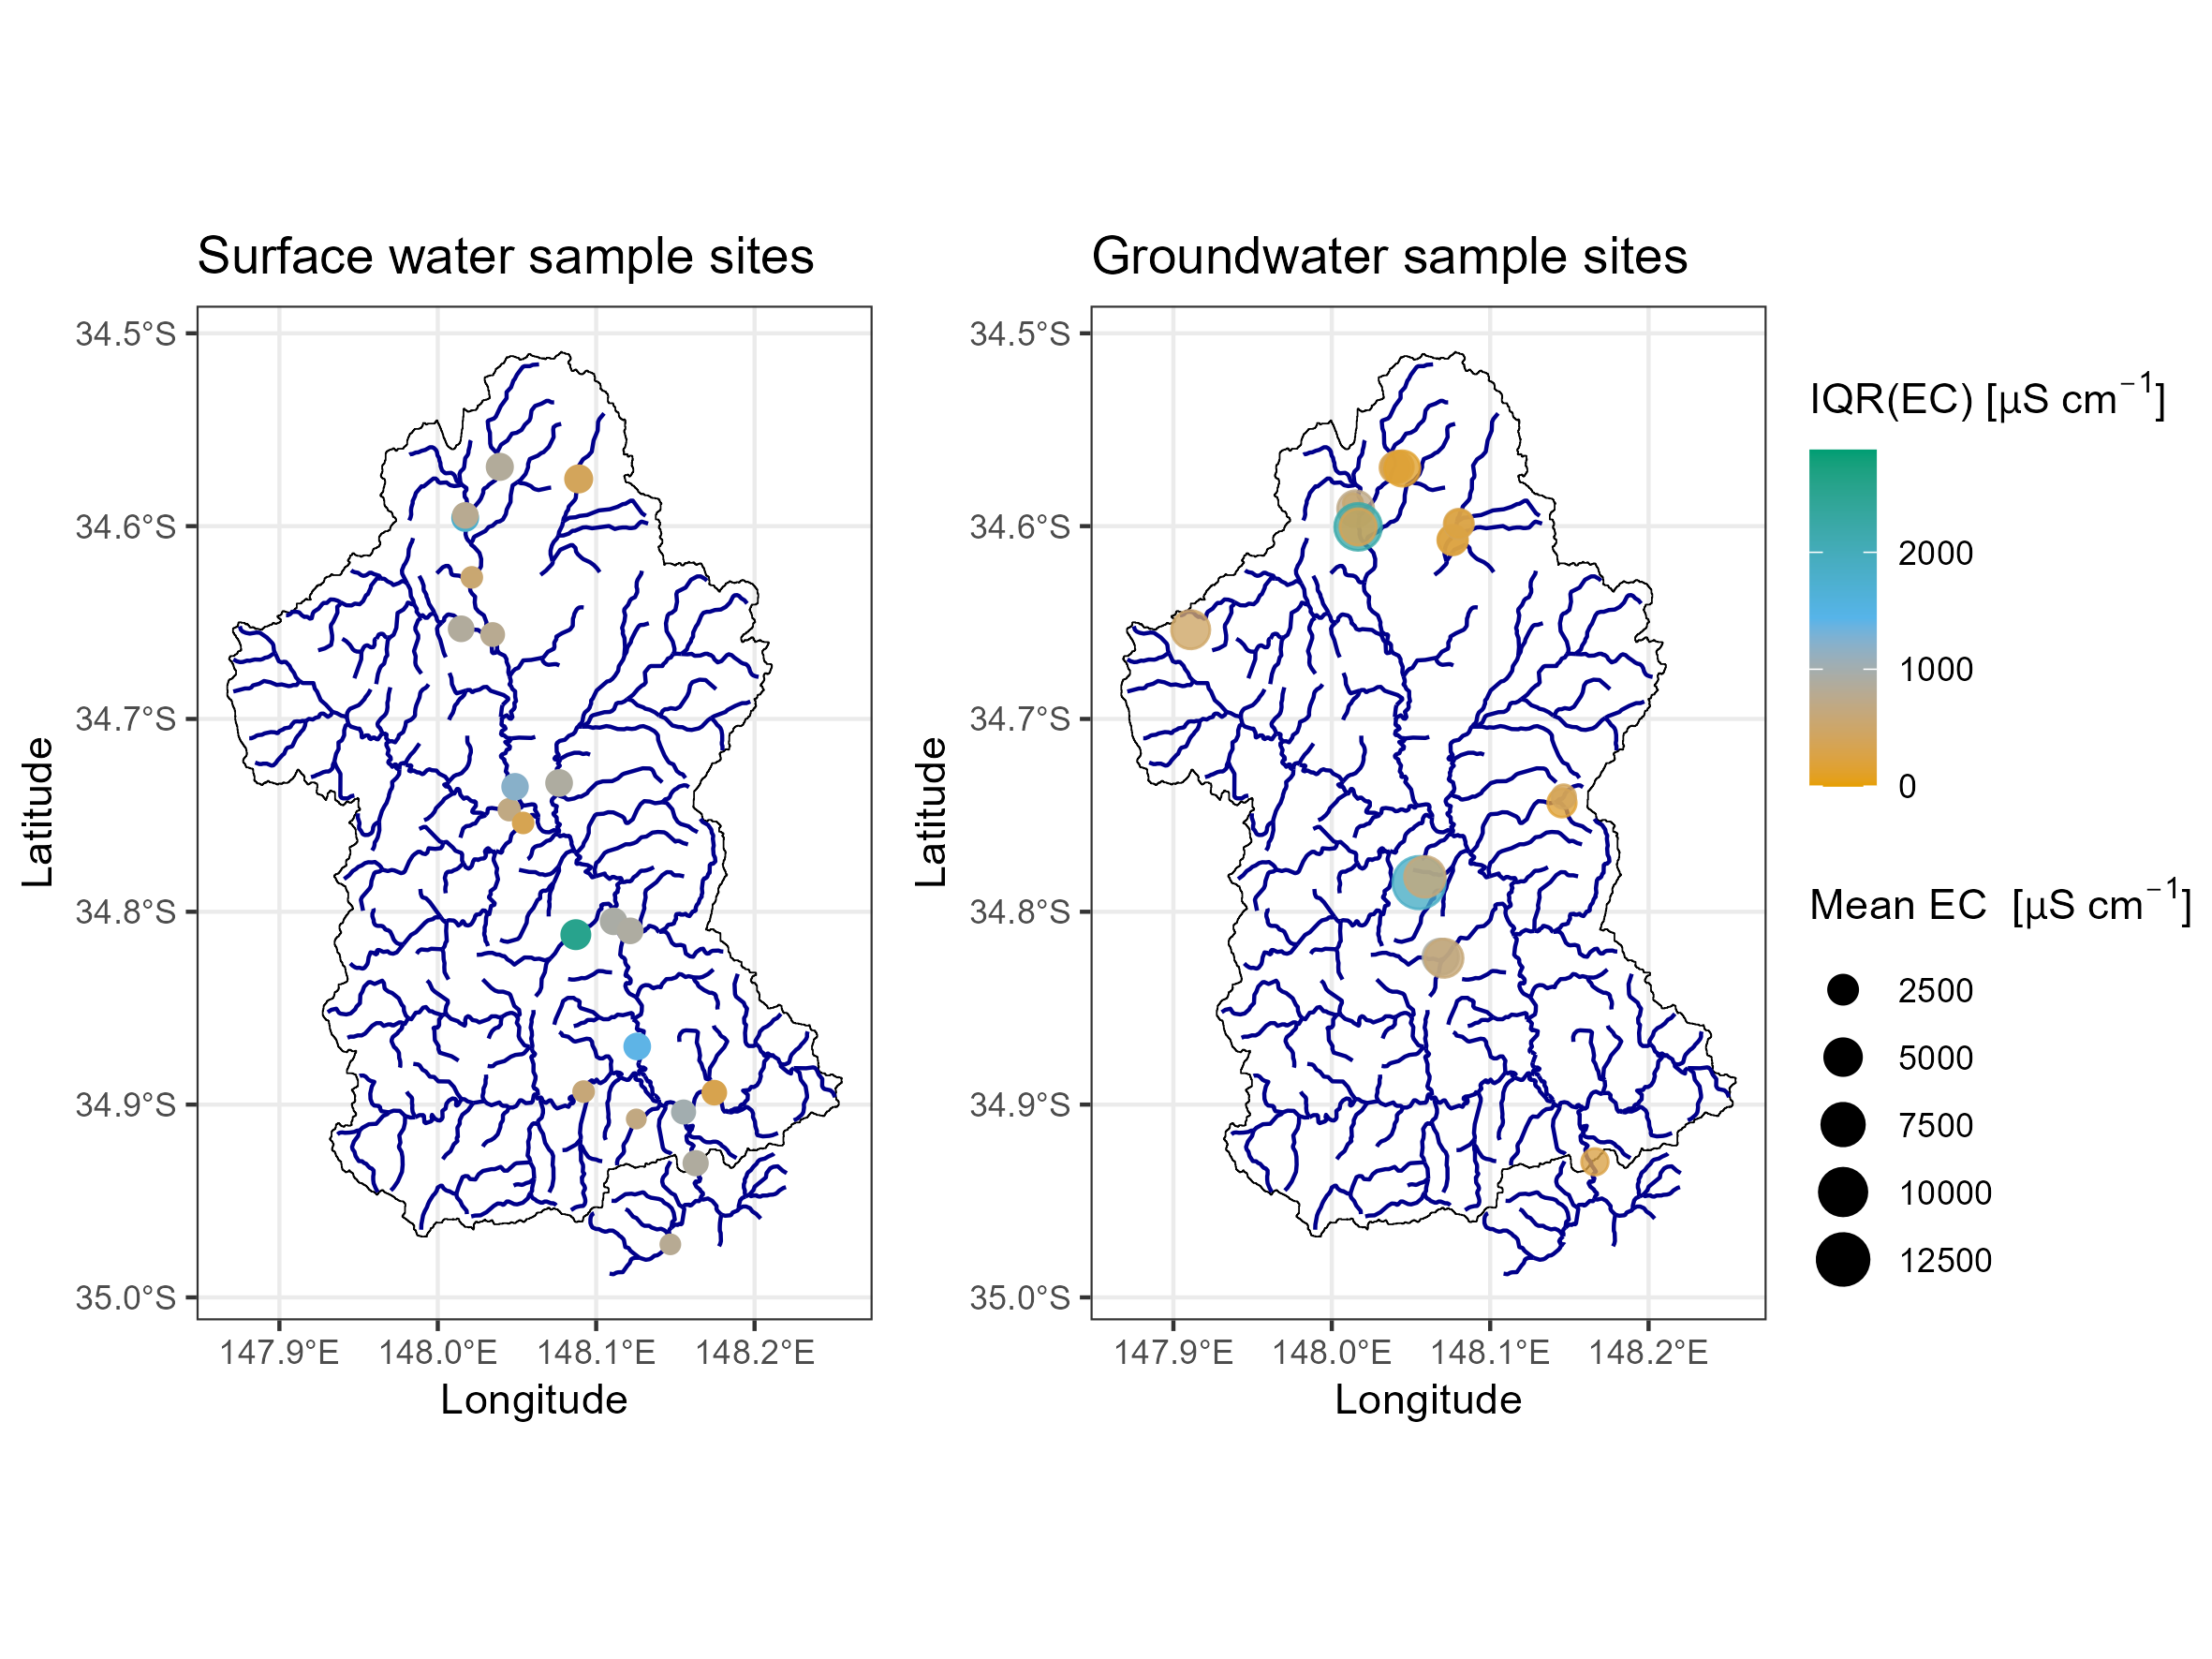
\includegraphics[width=0.8\linewidth]{Figures/ec_map} \caption{Spatial Variation of EC throughout the catchment, using Mean EC for each sampling location}\label{fig:ECmap}
\end{figure}

\begin{figure}
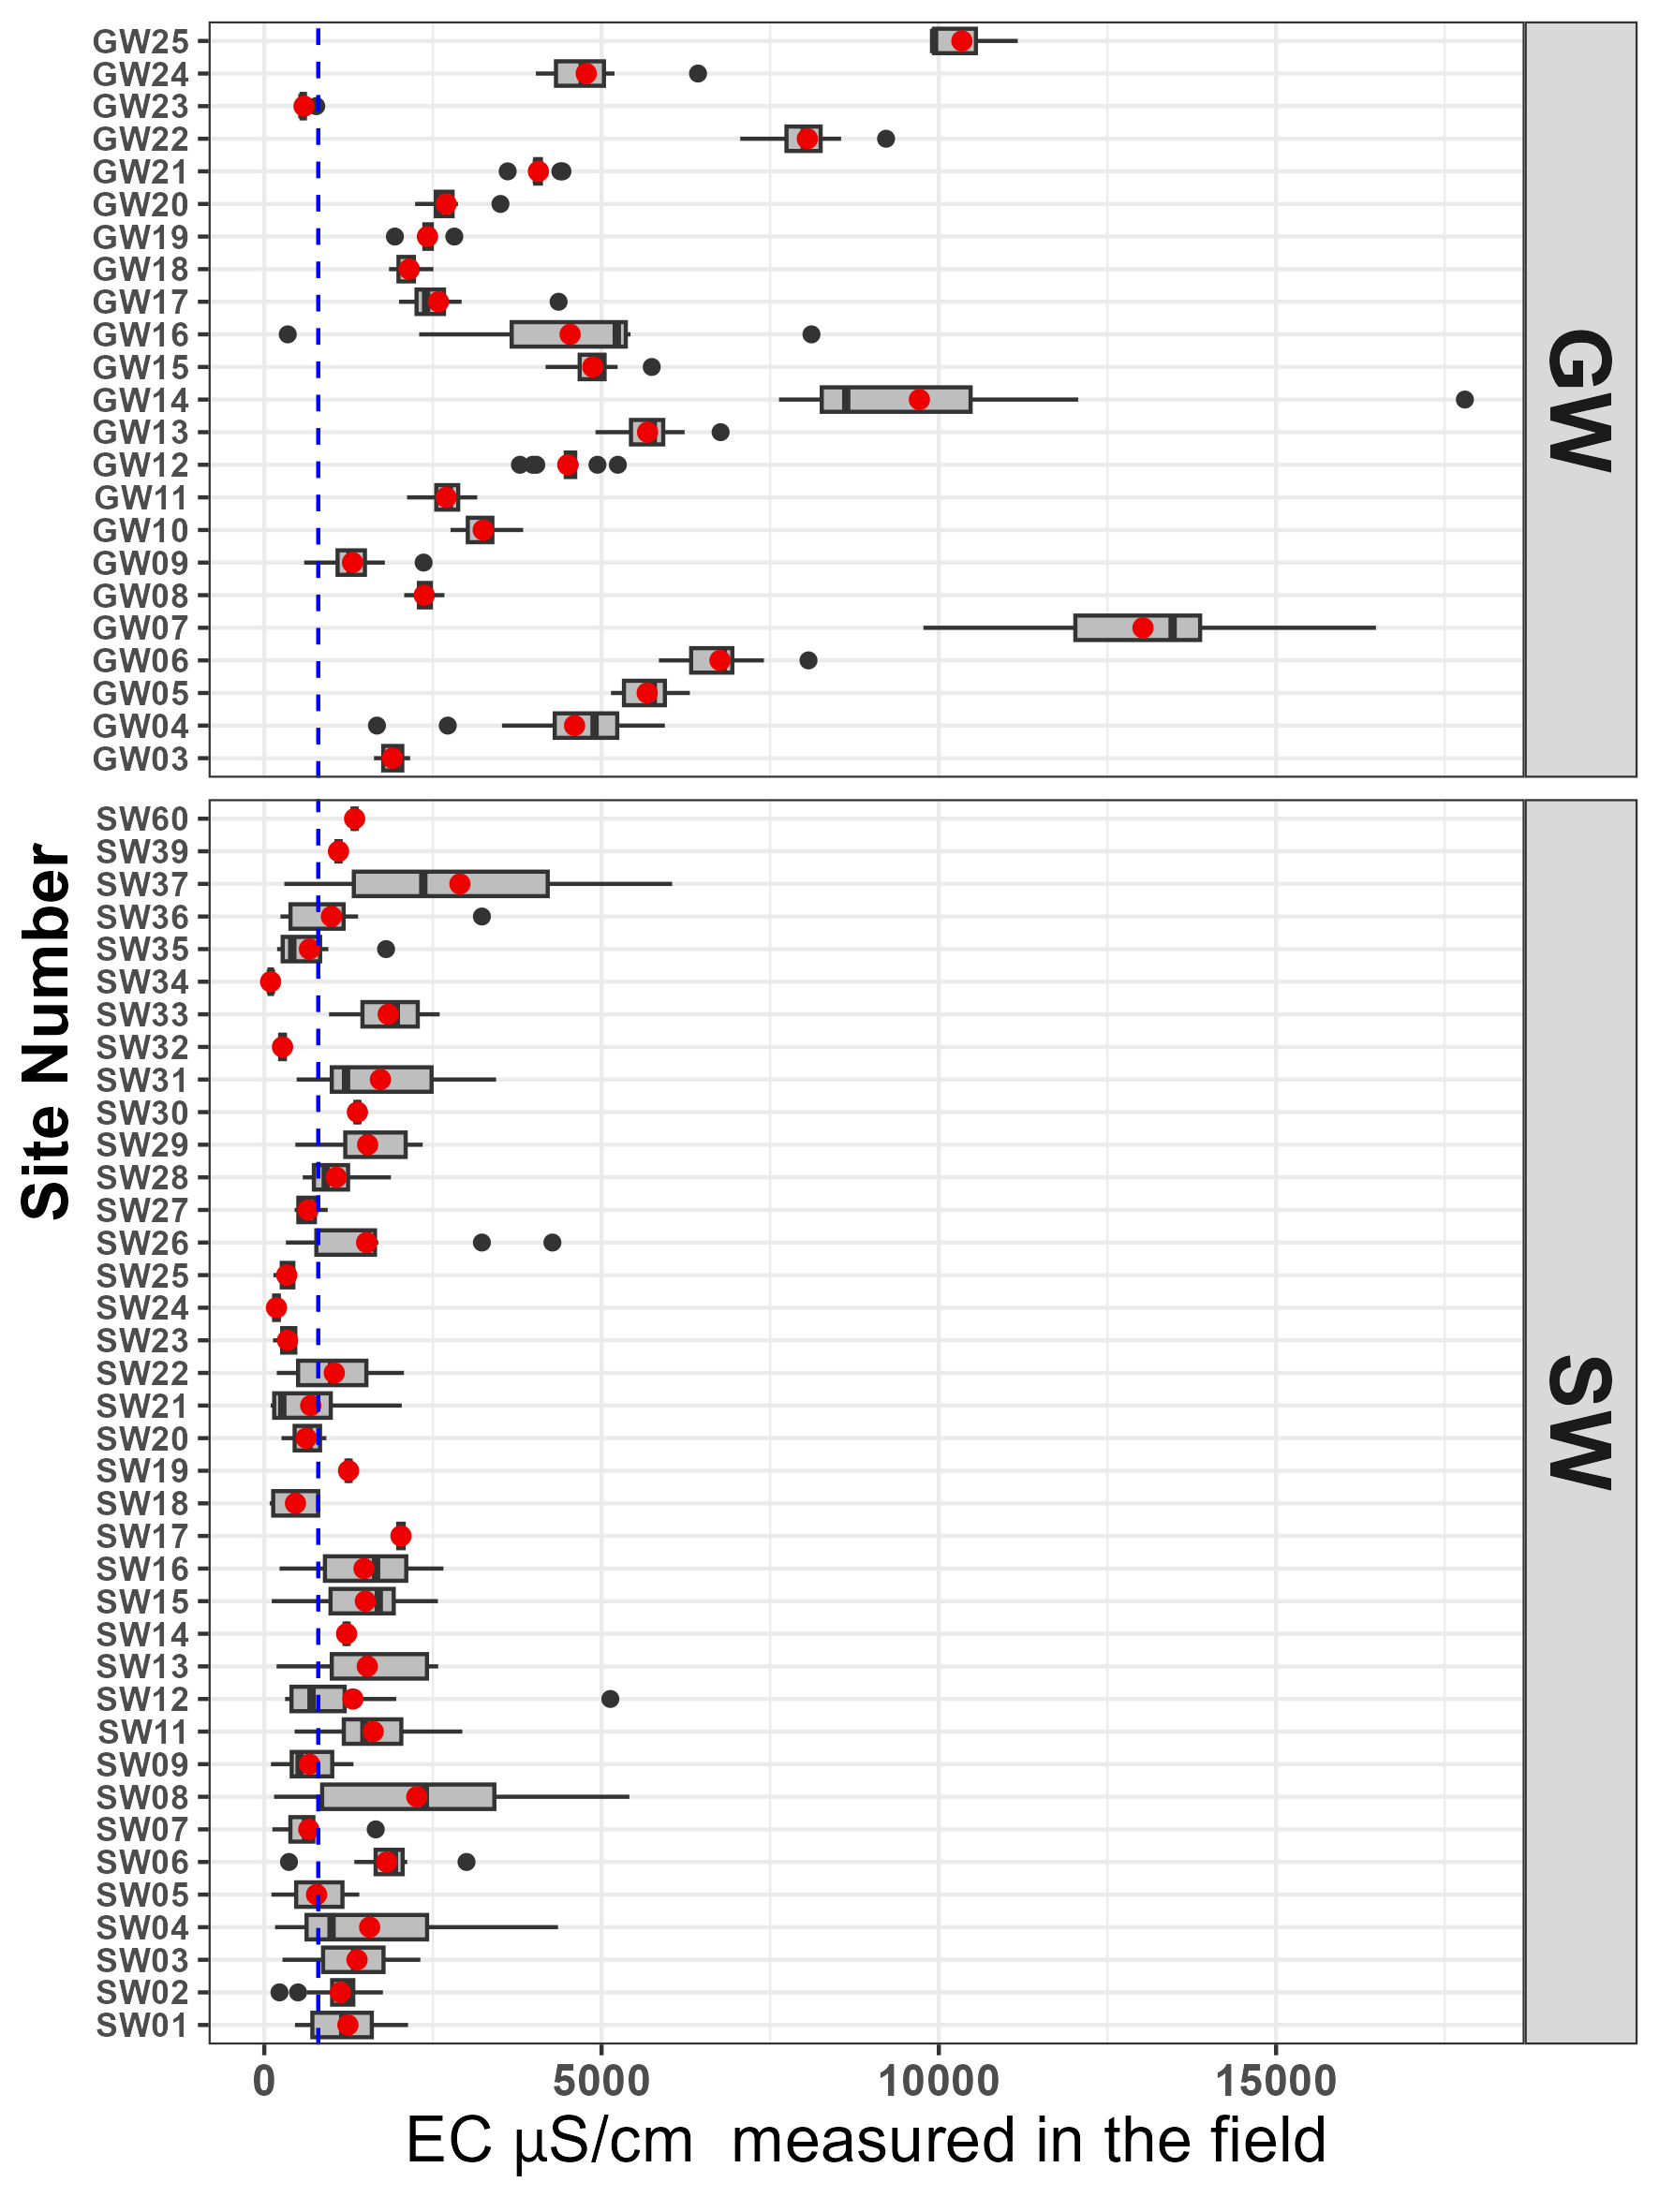
\includegraphics[width=0.8\linewidth]{Figures/ec_plot} \caption{Variation in EC throughout the catchment and in time by sample location}\label{fig:ECboxplot}
\end{figure}

\clearpage
\begin{figure}
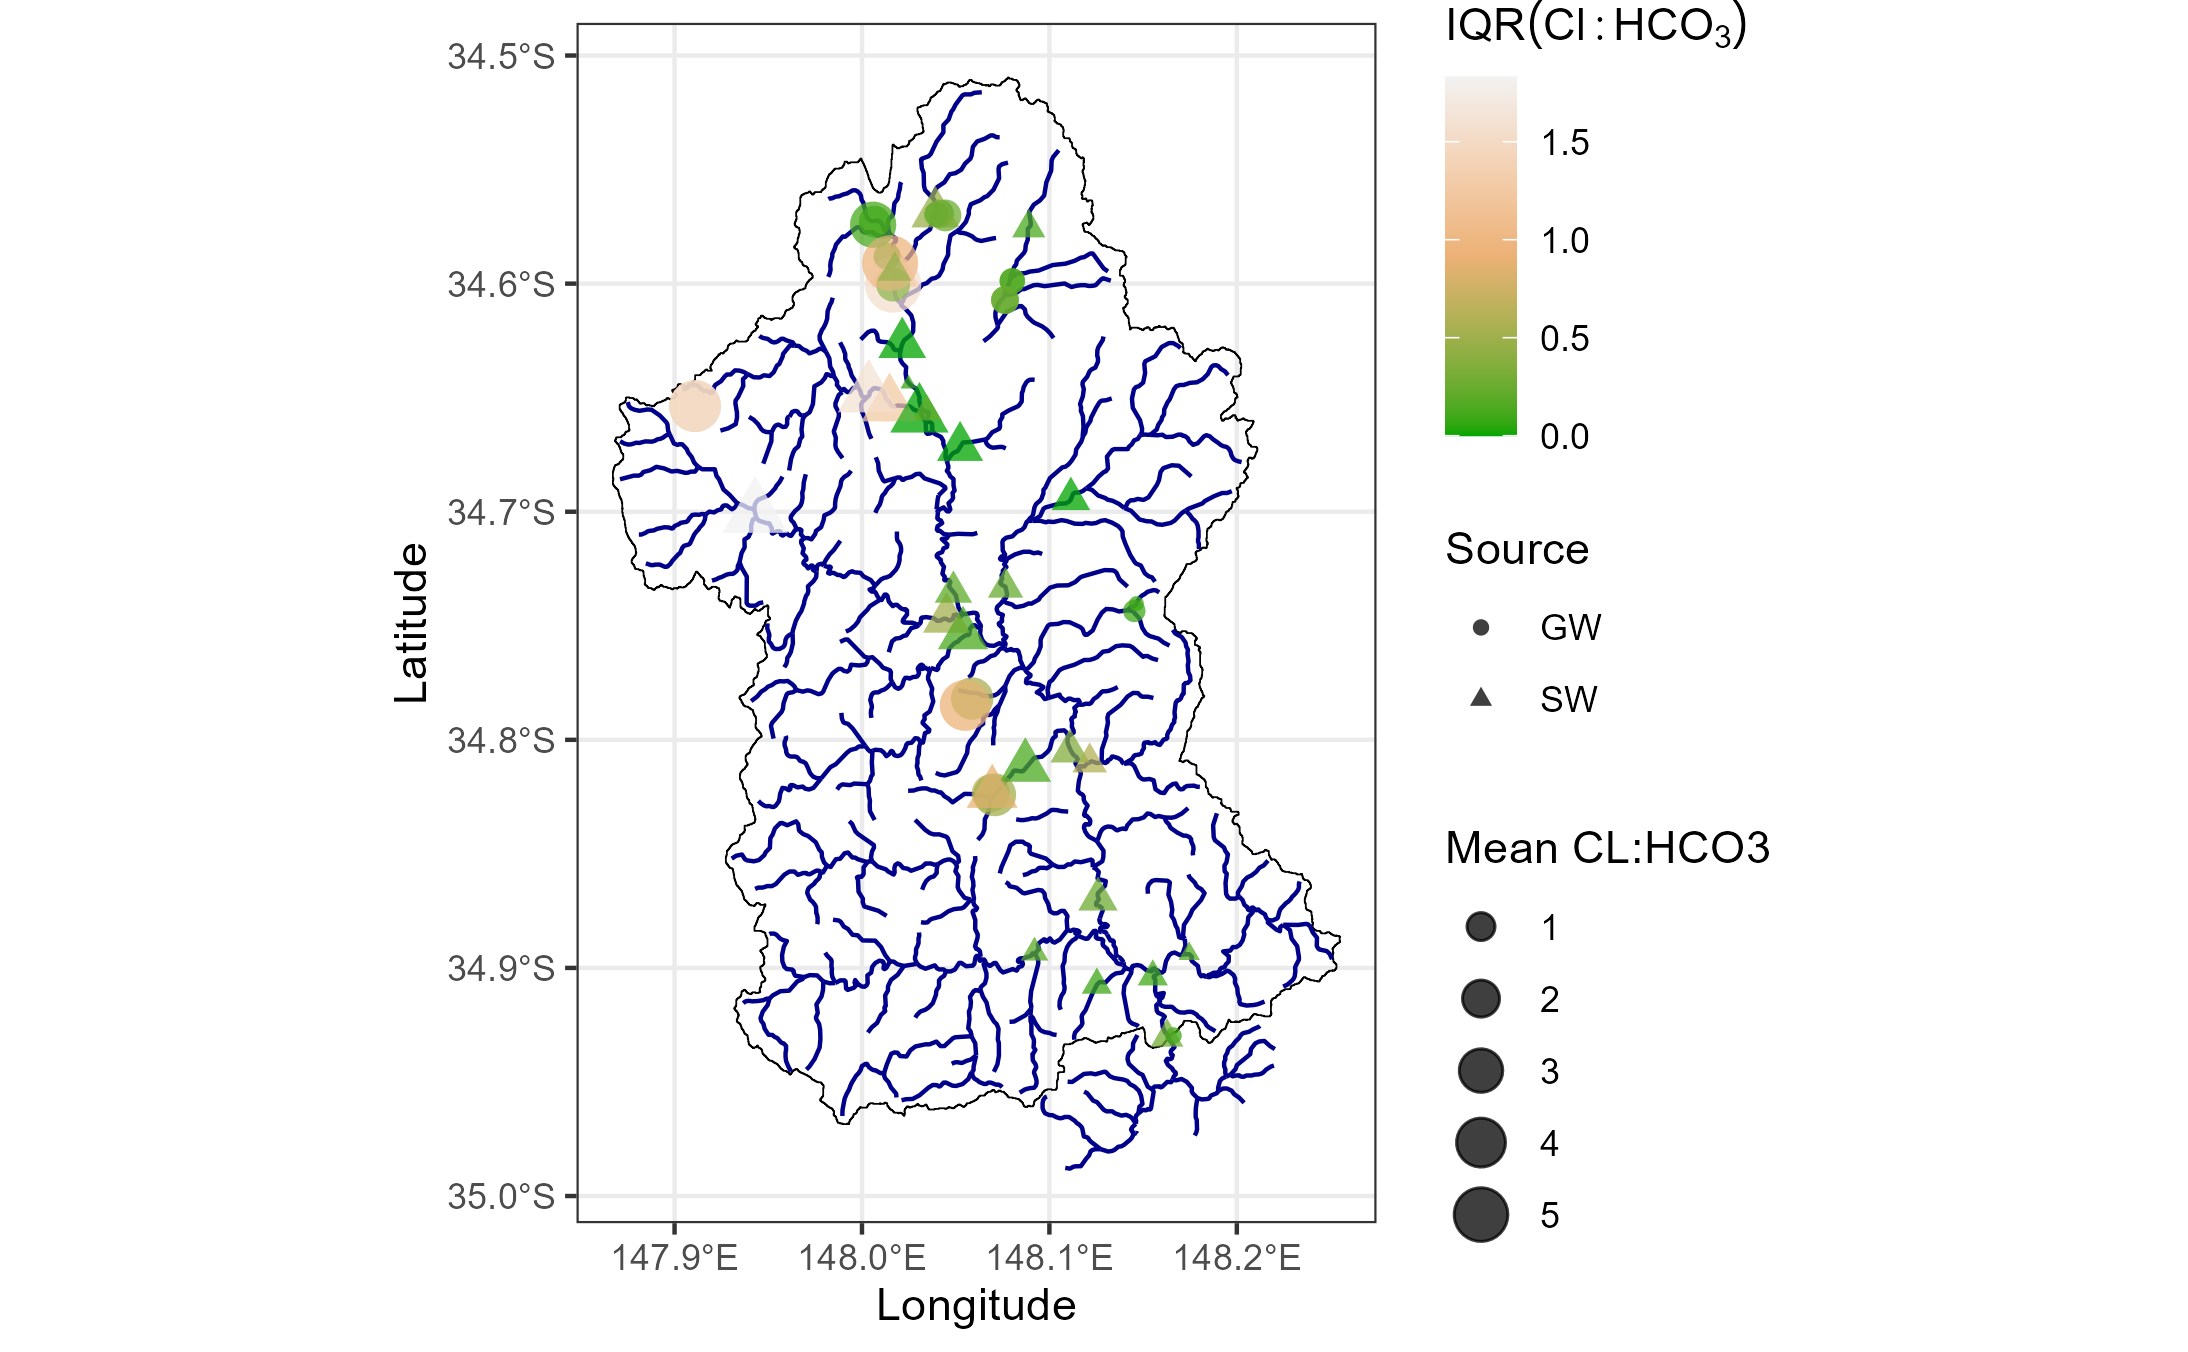
\includegraphics[width=0.8\linewidth]{Figures/clhco3_map} \caption{Spatial Variation of Cl:HCO3 ratio throughout the catchment, using Mean for each sampling location.}\label{fig:Carbonate-map}
\end{figure}

\begin{figure}
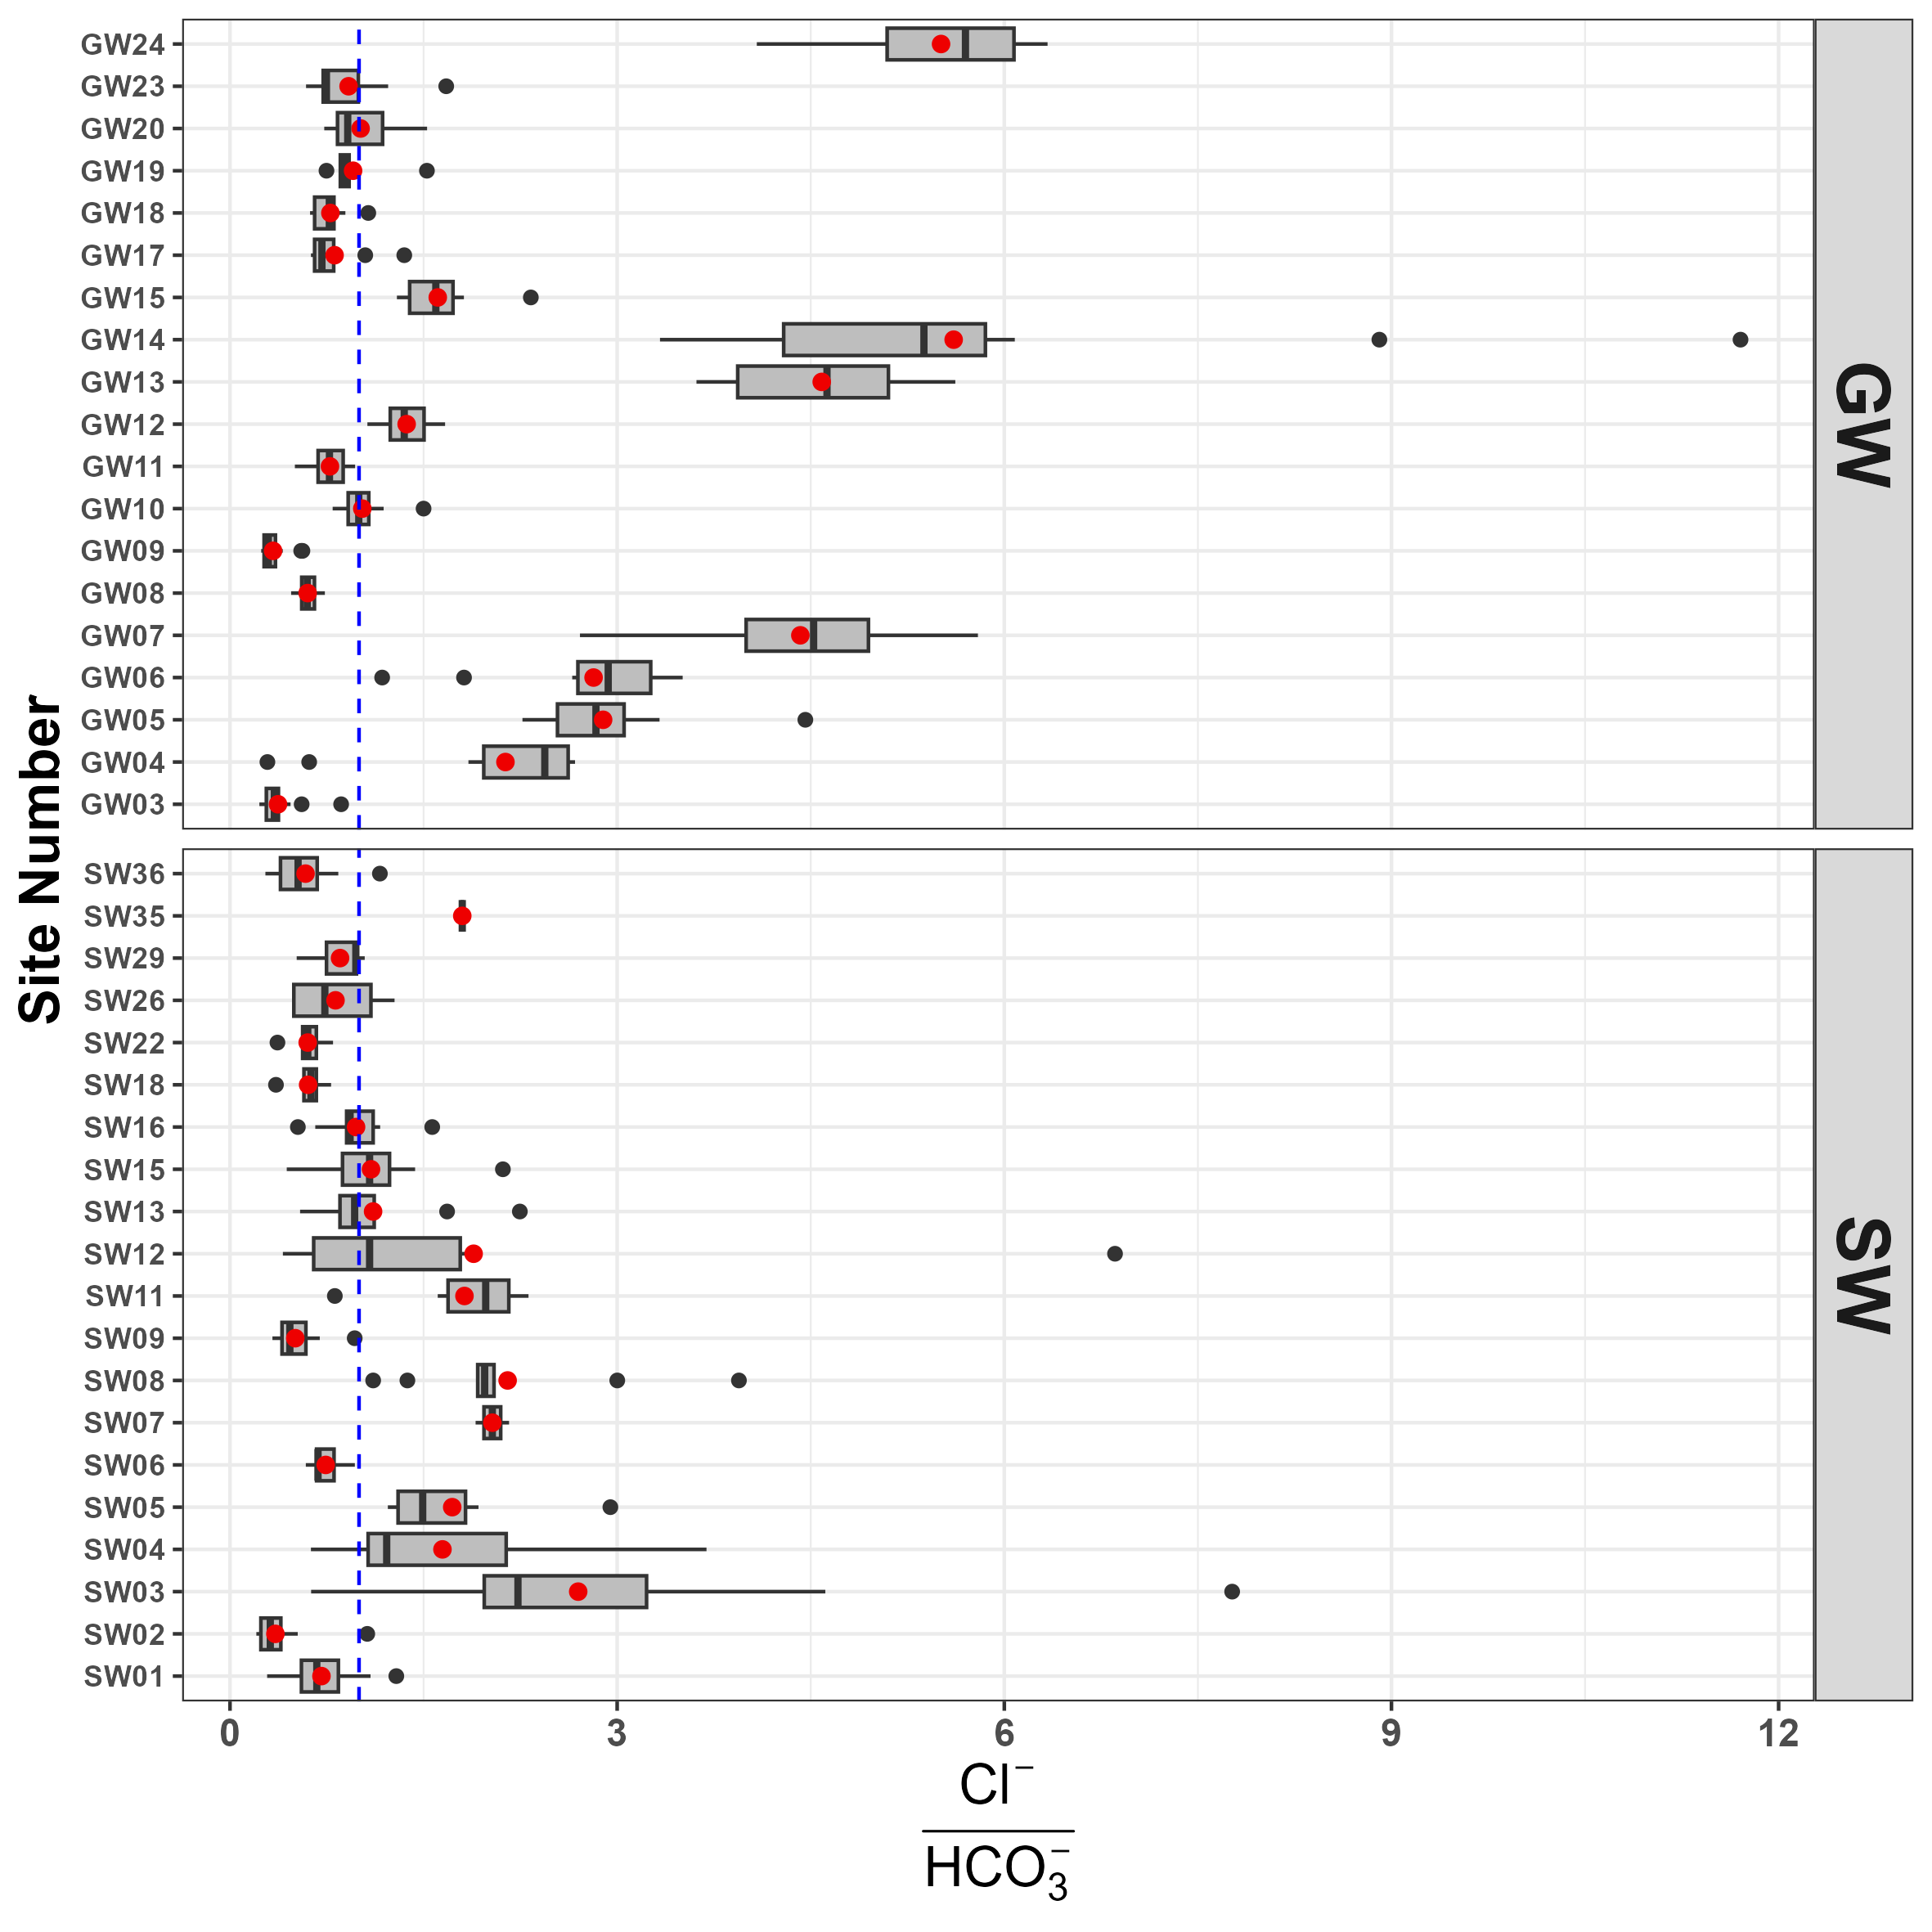
\includegraphics[width=0.8\linewidth]{Figures/clhco3_plot} \caption{Space and time Variation of Cl:HCO3 ratio by sampling location.}\label{fig:Carbonate-boxplot}
\end{figure}

There is clear spatial variation in water parameters throughout the
catchment, including between groundwater and surface water sampling
sites (Figures \ref{fig:ECmap} and \ref{fig:Carbonate-map}). As
examples, the spatial distributions for EC and Cl:HCO\textsubscript{3}
are shown, as well as the space time boxplots for the variables. Similar
maps can be easily generated for other parameters using the code in the
supplementary material. In the map, the concentration is indicated by
the size of the symbol, while the colour shading indicates the
variability. This suggests surface water samples had lower variability
and lower concentrations. Below the maps, a boxplot (Figures
\ref{fig:ECboxplot} and \ref{fig:Carbonate-boxplot}) further indicates
the difference in the distributions from the surface water sample sites
and the groundwater sample sites, and indicates the difference between
sample sites.

Previous studies have suggested there may be a difference in
Cl:HCO\textsubscript{3} ratio in surface water between the eastern and
western parts of the Muttama catchment \citep{Conyers2008}, however it
is difficult to see whether this pattern occurs based on the spatial
maps. This partly has to do with the limitations in the spatial
sampling, which relied on existing groundwater tube wells and accessible
stream points.

\subsection{Principal Component Analysis (PCA)}

\clearpage
\begin{figure}
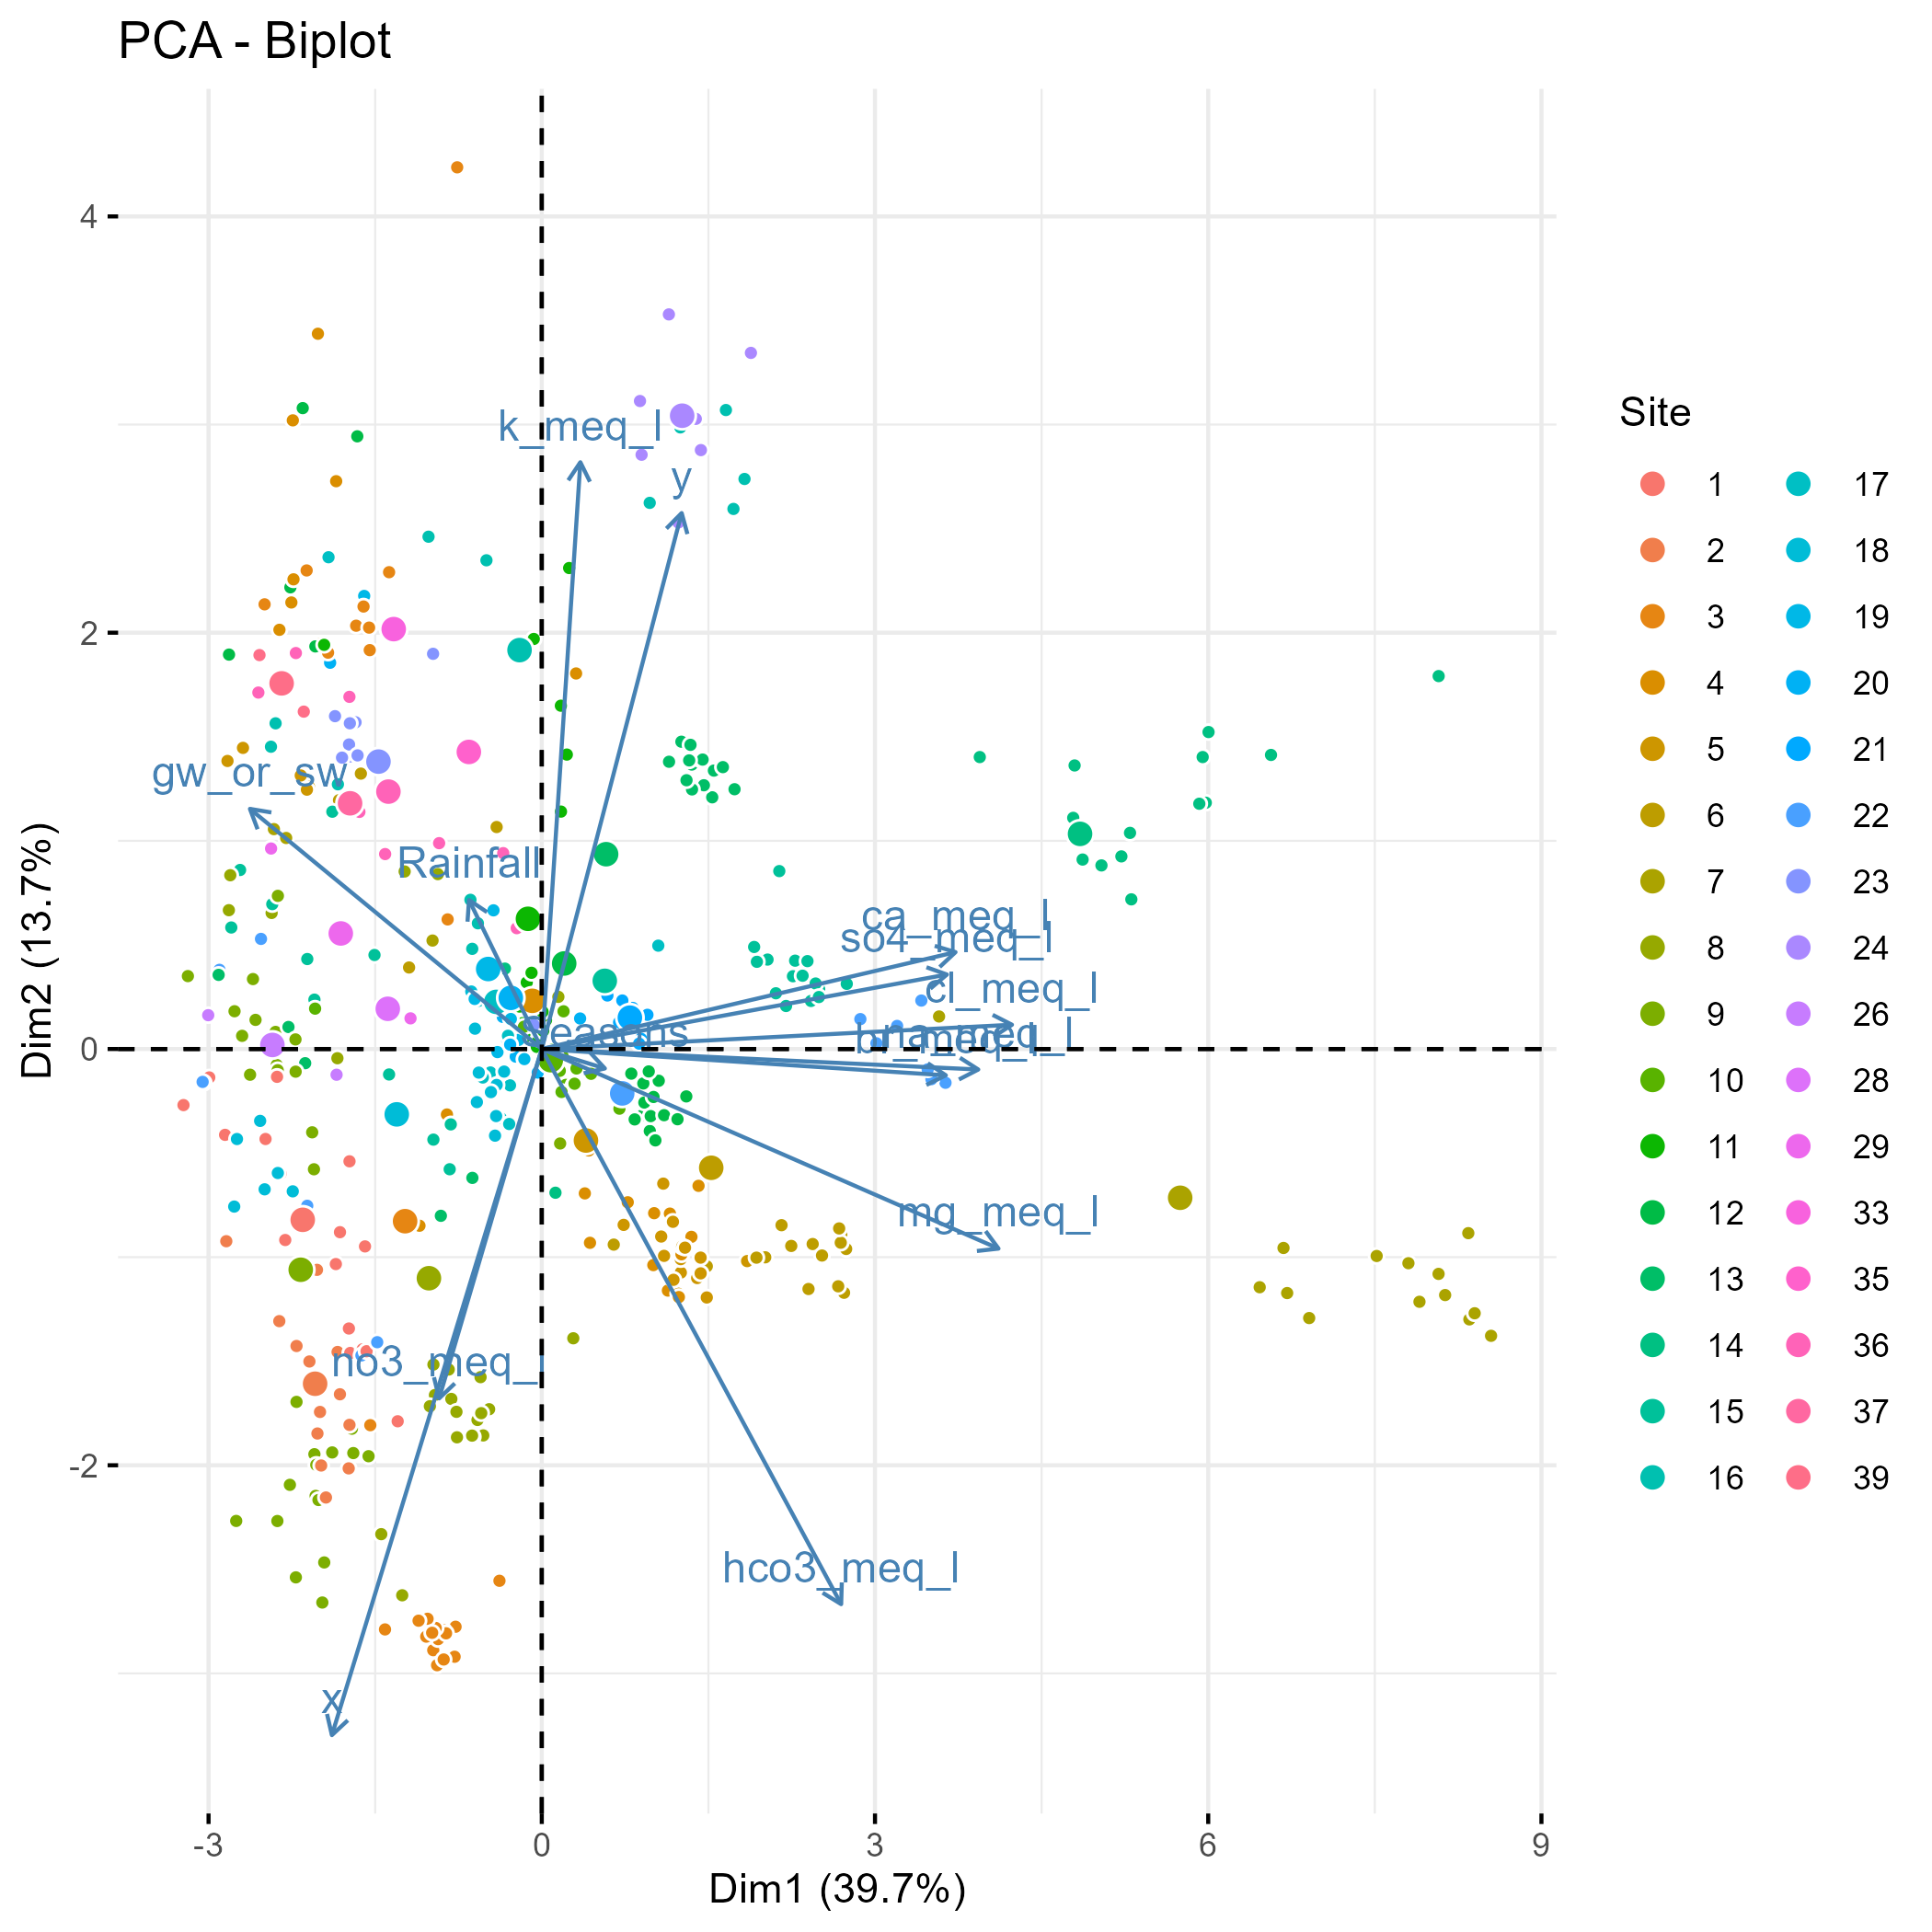
\includegraphics[width=0.9\linewidth]{Figures/pca_biplot} \caption{PCA Biplot of the data. Missing values were removed from the data resulting in a reduced data set}\label{fig:PCA-plot}
\end{figure}

The results of the PCA (Fig \ref{fig:PCA-plot}) highlights that location
is the most important determinant of the characteristics of a sample.
Coordinates and whether the sample originates from groundwater or
surface water (gw\_or\_sw) explains most of the variation. Rainfall and
Seasons (numerical, 1 = Spring, 4 = Winter) do not appear to have much
of an effect, suggesting that the variation in time in the data is
smaller than the variation in space. This could be partly because we
have lumped groundwater and surface water samples together, and the
variation in the surface water samples is masked by the more stationary
nature of the groundwater concentrations.

Most salt species are grouped together, apart from potassium (K),
magnesium (Mg), nitrates (NO\textsubscript{3}) and bicarbonates
(HCO\textsubscript{3}). This suggests that these variables (K, Mg,
NO\textsubscript{3} and HCO\textsubscript{3}) are the main parameters
that will separate the samples. Given that HCO\textsubscript{3} and Mg
are negatively correlated with the gw\_or\_sw variable, this suggests
that groundwater samples are higher in Mg and HCO\textsubscript{3}
compared to surface water samples. In contrast NO\textsubscript{3} and K
are associated with the spatial variables x and y, thus suggesting some
spatial pattern in the samples.

\section{Conclusions}

This paper reports on a long term (10 year) hydrogeochemistry dataset
from a single catchment in NSW, Australia. This dataset includes both
groundwater and surface water samples for 0 locations within the
catchment. While the dataset was collected by different groups of people
at different times and locations, it still provides a valuable long term
and spatially diverse data set which can be used for research into the
space and time variation in dryland and groundwater salinity.



\codedataavailability{add a GitHub and cloudstor
repos} %% use this section when having data sets and software code available



%%%%%%%%%%%%%%%%%%%%%%%%%%%%%%%%%%%%%%%%%%
%% optional

%%%%%%%%%%%%%%%%%%%%%%%%%%%%%%%%%%%%%%%%%%
\appendix
\section{Figures and tables in appendices}
\noappendix

%%%%%%%%%%%%%%%%%%%%%%%%%%%%%%%%%%%%%%%%%%
\authorcontribution{T. Bishop initiated the sampling campaign. T.
Bishop, F. van Ogtrop and R.W. Vervoort conceptualised the overall
study. R.W. Vervoort and M. Tambrchi wrote the paper and analysed
results. F.Akter and J. Lessels collected and analysed the majority of
the samples. M. Tambrchi, A. Buzacott, J. Moloney, F. Akter analysed and
managed the data. All authors participated in sampling, laboratory
analysis and review of the paper.} %% optional section

%%%%%%%%%%%%%%%%%%%%%%%%%%%%%%%%%%%%%%%%%%
\competinginterests{The authors declare no competing
interests.} %% this section is mandatory even if you declare that no competing interests are present

%%%%%%%%%%%%%%%%%%%%%%%%%%%%%%%%%%%%%%%%%%

%%%%%%%%%%%%%%%%%%%%%%%%%%%%%%%%%%%%%%%%%%
\begin{acknowledgements}
This dataset would not have been possible without the generous
assistance and access to properties from the following land owners in
the Muttama Creek area: R. Last, the Tozer family, M. Sullivan, P.
McClintock, P. McGuire, S. Sharman, A. Hollihan, the managers at Brawlin
Springs as part of the Romani Pastoral Company, and the managers and
owners of Wavehill, in particular J. Litchfield. We would like to thank
several generations of students in the units LWSC2002, ENVX3003 and
ENSY5708, as well a multiple interns from French Institutions and
University and Wageningen University for assisting with the sample
collection.
\end{acknowledgements}

%% REFERENCES
%% DN: pre-configured to BibTeX for rticles

%% The reference list is compiled as follows:
%%
%% \begin{thebibliography}{}
%%
%% \bibitem[AUTHOR(YEAR)]{LABEL1}
%% REFERENCE 1
%%
%% \bibitem[AUTHOR(YEAR)]{LABEL2}
%% REFERENCE 2
%%
%% \end{thebibliography}

%% Since the Copernicus LaTeX package includes the BibTeX style file copernicus.bst,
%% authors experienced with BibTeX only have to include the following two lines:
%%
\bibliographystyle{copernicus}
\bibliography{datapaper.bib}
%%
%% URLs and DOIs can be entered in your BibTeX file as:
%%
%% URL = {http://www.xyz.org/~jones/idx_g.htm}
%% DOI = {10.5194/xyz}


%% LITERATURE CITATIONS
%%
%% command                        & example result
%% \citet{jones90}|               & Jones et al. (1990)
%% \citep{jones90}|               & (Jones et al., 1990)
%% \citep{jones90,jones93}|       & (Jones et al., 1990, 1993)
%% \citep[p.~32]{jones90}|        & (Jones et al., 1990, p.~32)
%% \citep[e.g.,][]{jones90}|      & (e.g., Jones et al., 1990)
%% \citep[e.g.,][p.~32]{jones90}| & (e.g., Jones et al., 1990, p.~32)
%% \citeauthor{jones90}|          & Jones et al.
%% \citeyear{jones90}|            & 1990


\end{document}
